\documentclass[journal,twoside,web]{ieeecolor}

\usepackage{xcolor}

% amsmath and amssymb packages, useful for mathematical formulas and symbols
\usepackage{amsmath,amssymb}
\usepackage{generic}

% Use Unicode characters when possible
\usepackage[utf8x]{inputenc}


% Use nameref to cite supporting information files (see Supporting Information section for more info)
\usepackage{nameref,hyperref}

% line numbers
% \usepackage[right]{lineno}

% color can be used to apply background shading to table cells only
%\usepackage[table]{xcolor}

% array package and thick rules for tables
\usepackage{array}

\usepackage{booktabs}
% \usepackage[colorlinks=TRUE,linkcolor=olive,citecolor=brown]{hyperref}


\usepackage{bm}
% \usepackage{caption}

% \usepackage{todonotes}


\usepackage[resetlabels]{multibib}
\newcites{app}{Appendix References}

\newtheorem{fact}{Fact}[section]
\newtheorem{lemma}[fact]{Lemma}
\newtheorem{theorem}[fact]{Theorem}
\newtheorem{definition}[fact]{Definition}
\newtheorem{corollary}[fact]{Corollary}
\newtheorem{proposition}[fact]{Proposition}
\newtheorem{claim}[fact]{Claim}
\newtheorem{exercise}[fact]{Exercise}
\newtheorem{remark}[fact]{Remark}

\usepackage{algorithm}
\usepackage{algorithmic}

\usepackage{graphicx}
% \usepackage{setspace}
% \doublespace

% Bold the 'Figure #' in the caption and separate it from the title/caption with a period
% Captions will be left justified
% \usepackage[aboveskip=1pt,labelfont=bf,labelsep=period,justification=raggedright,singlelinecheck=off]{caption}

\usepackage{subcaption}

% \usepackage[numbers]{natbib}
% \setcitestyle{citesep={;}}
% \usepackage{changes}


% \renewcommand{\figurename}{Fig}


% Leave date blank
\date{}



\renewcommand{\Re}{\mathbb{R}}

\newcommand{\Ex}{\mathbb{E}}

\renewcommand{\algorithmicrequire}{\textbf{Input:}} 
\renewcommand{\algorithmicensure}{\textbf{Output:}} 
%\renewcommand{\hat}{\widehat}


\begin{document}


\title{Connectome Smoothing via Low-rank Approximations}
\author{Runze Tang,
Michael Ketcha,
Alexandra Badea, 
Evan D.~Calabrese,\\
Daniel S. Margulies,
Joshua T.~Vogelstein,
Carey E.~Priebe~\IEEEmembership{Senior Member,~IEEE},
Daniel L.~Sussman%
% \IEEEcompsocitemizethanks{
\thanks{
Submitted on March 28, 2018.
This work is graciously supported by the XDATA program of the Defense
Advanced Research Projects Agency (DARPA) administered through Air
Force Research Laboratory contract FA8750-12-2-0303; the DARPA SIMPLEX
program through SPAWAR contract N66001-15-C-4041; and DARPA GRAPHS
contract N66001-14-1-4028. We would also like to acknowledge support from NIH through K01 AG041211, and P41 EB015897.}
\thanks{R. Tang and C. E. Priebe are with the Department of Applied Math \& Statistics, The Johns Hopkins University, Baltimore, MD}
\thanks{M. Ketcha and J. T. Vogelstein are with the Department of Biomedical Engineering,  The Johns Hopkins University, Baltimore, MD}
\thanks{A. Badea and E. D.~Calabrese are with the Department of Radiology, and Department of Biomedical Engineering, Duke University, Durham, NC}
\thanks{D. S. Margulies is with Max Planck Research Group for Neuroanatomy \& Connectivity, Max Planck Institute for Human Cognitive and Brain Sciences, Leipzig, Germany}
\thanks{J. T. Vogelstein is also with Child Mind Institute, New York City, NY}
\thanks{D. L. Sussman is with the Department of Mathematics \& Statistics, Boston University, Boston, MA; e-mail: sussman@bu.edu}}




% Title must be 250 characters or less.

% Insert author names, affiliations and corresponding author email (do not include titles, positions, or degrees).

% The author names are missing -Toni



\maketitle



% Please keep the abstract below 300 words
\begin{abstract}
In statistical connectomics, the study of brain networks, estimating the mean of a population of graphs based on a sample is a core problem.
Often, this problem is especially difficult because the sample or cohort size is relatively small, sometimes even a single subject.
While using the element-wise sample mean of the adjacency matrices is a common approach, this method does not exploit underlying structural properties of the graphs.
We propose using a low-rank method which incorporates dimension selection and diagonal augmentation to smooth the estimates and improve performance over the na\"ive methodology for small sample sizes.
Theoretical results for the stochastic blockmodel show that this method offers major improvements when there are many vertices.
Similarly, we demonstrate that the low-rank methods outperform the standard sample mean for a variety of independent edge distributions as well as human connectome data derived from magnetic resonance imaging, especially when sample sizes are small.
Moreover, the low-rank methods yield ``eigen-connectomes'', which correlate with the lobe-structure of the human brain and superstructures of the mouse brain.
These results indicate that low-rank methods are an important part of the toolbox for researchers studying populations of graphs in general, and statistical connectomics in particular.
\end{abstract}
\begin{IEEEkeywords}
networks, connectome, low-rank, estimation
\end{IEEEkeywords}


% To allow for easy dual compilation without having to reenter the
% abstract/keywords data, the \IEEEtitleabstractindextext text will
% not be used in maketitle, but will appear (i.e., to be "transported")
% here as \IEEEdisplaynontitleabstractindextext when the compsoc 
% or transmag modes are not selected <OR> if conference mode is selected 
% - because all conference papers position the abstract like regular
% papers do.
% \IEEEdisplaynontitleabstractindextext has no effect when using
% compsoc or transmag under a non-conference mode.



% For peer review papers, you can put extra information on the cover
% page as needed:
% \ifCLASSOPTIONpeerreview
% \begin{center} \bfseries EDICS Category: 3-BBND \end{center}
% \fi
%
% For peerreview papers, this IEEEtran command inserts a page break and
% creates the second title. It will be ignored for other modes.
% \IEEEpeerreviewmaketitle

\section{Introduction}\label{sec:intro}

In this manuscript we consider the challenges of estimating a population mean based on a sample of brain networks, as represented by their structural connectomes.
Estimation of the mean of a population based on samples is at the core of statistics.
The sample mean, motivated by its intuitive appeal, the law of large numbers, and the central limit theorem, has its place as one of the most important statistics for this task.
% In modern settings, averages of many different kinds of data representations are taken, including scalars and vectors, but also objects  like images, shapes, and documents.

However, the mean of a population of graphs is a high-dimensional object, consisting of $O(N^2)$ parameters for graphs with $N$ nodes (vertices).
When the number of samples $M$ is much smaller than $N^2$, or even $N$, estimating such a high-dimensional estimands using naive unbiased methods can lead to inaccurate estimates with very high variance.
Furthermore, using these estimates for subsequent inference tasks such as testing can lead to low power and accuracy.
By exploiting a bias-variance trade-off, it is often fruitful to develop estimators which have some bias but greatly reduced variance.
When these estimators are biased towards low-dimensional structures which well approximate the full dimensional population mean, major improvements in estimation can be realized \cite{trunk1979problem}.
Furthermore, a more parsimonious representation of the mean improves interpretability and allows for novel exploratory analyses.
% \todo{fix}Many literatures focus on the low-dimensional representation, for example \cite{allard2012multi} constructs data-dependent multi-scale dictionaries that aim at efficient encoding and manipulating of the data.



In complex data settings such as shape data, language data, or graph data, caution is necessary even in properly defining the mean.
For a population, we define the mean graph as the weighted adjacency matrix with weights given by the proportion of times the corresponding edge appears in the population.
This definition naturally extends the definition of the mean for standard Euclidean data.
As with real valued data, one may want to define the mean of a population of graphs to be a graph.
This is captured in the notion of the median graph \cite{jiang2001median}. However, this may be too restrictive for populations of graphs where there is high variation.
As described below, our definition of the mean graph is the expectation of the adjacency matrix.

The population mean is becoming an important object for statistical connectomics applications.
For example, \cite{ginestet2014hypothesis} proposed a way to test if there is a difference between the distributions for two groups of networks.
While hypothesis testing is the end goal of their work, estimation is a key intermediate step which may be improved by accounting for underlying structure in the mean matrix.
Thus, improving the estimation procedures for the mean graph is not only important by itself, but also can be applied to help improve other statistical inference procedures.

To better illustrate the idea, consider  brain graphs (connectomes) available through the Consortium for Reliability and Reproducibility (CoRR) \cite{zuo2014open} after processing with ndmg pipeline \cite{kiar2017science, kiar2016ndmg}.
In particular, the SWU4 dataset contains 454 brain scans \cite{SWU4}.
Each vertex in the estimated graphs represents a region defined by the Desikan atlases, while an edge exists between two vertices if there is at least one streamline connecting the corresponding regions of the brain.
More details about this dataset are given in Section \ref{sec:corr_data} and Section \ref{section:data}.
Our goal is to estimate the mean graph of the population $P$, defined as the entry-wise mean of all the 454 graphs. Fig.~\ref{fig:Matrix_desikan_m5} shows the population mean graph $P$ on the left panel.
Darker pixels indicate a higher proportion of graphs having an edge between the given vertices.



\begin{figure}[!tbp]
\centering
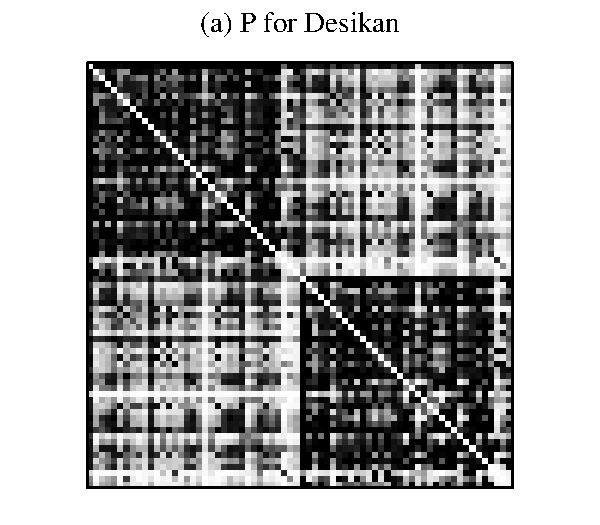
\includegraphics[height=.11\textheight]{P_desikan_m5.pdf} \hspace{-24pt}
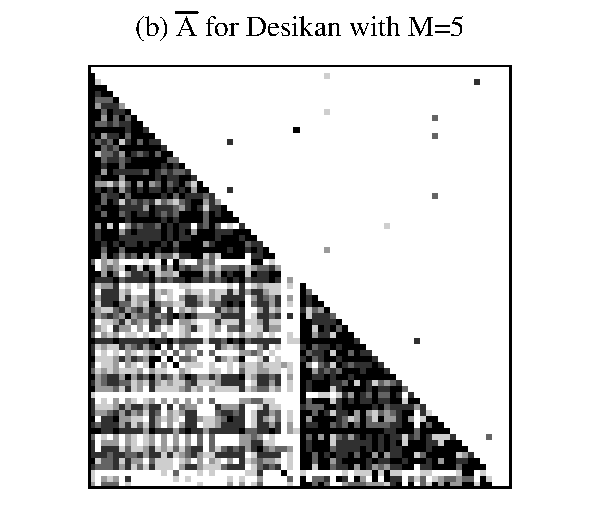
\includegraphics[height=.11005\textheight]{Abar_desikan_m5.pdf} \hspace{-24pt}
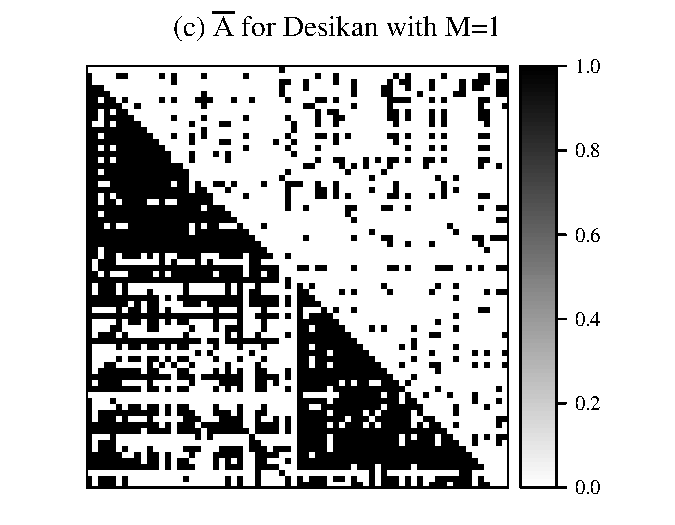
\includegraphics[height=.11005\textheight]{Abar_desikan_m1.pdf}
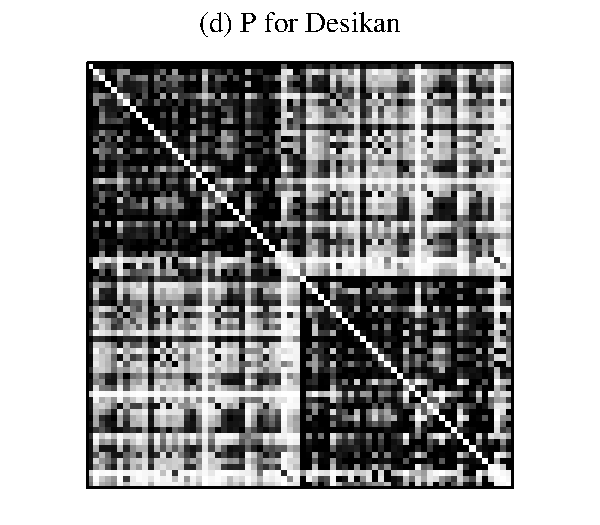
\includegraphics[height=.11\textheight]{P_desikan_m1.pdf} \hspace{-24pt}
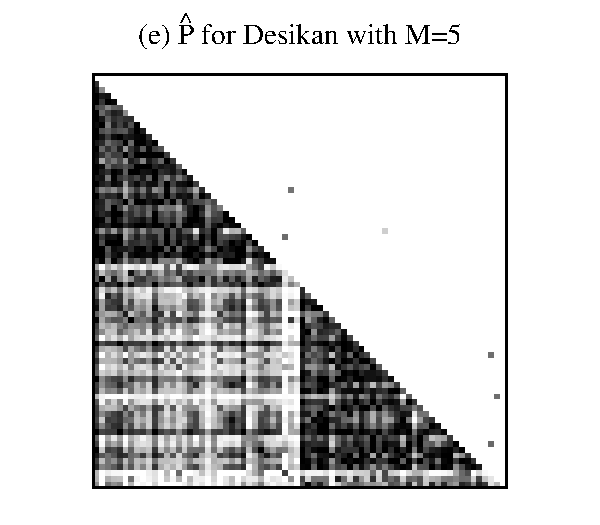
\includegraphics[height=.11025\textheight]{Phat_desikan_m5.pdf} \hspace{-24pt}
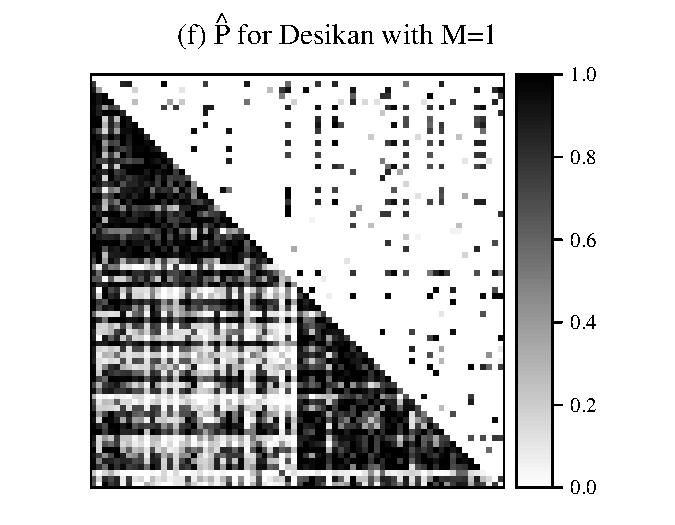
\includegraphics[height=.11025\textheight]{Phat_desikan_m1.pdf}
\caption{
% {\bf Heat maps estimands and estimates.}
The heat map of the population mean for the $454$ graphs are depicted in Panel (a) (also in Panel (d)).
The two heat maps in the second column indicate the sample mean for 5 sampled graphs (Panel (b)), and the low-rank estimate $\hat{P}$ for the same 5 sampled graphs with rank $d=11$ (Panel (e)), computed as described in Section~\ref{sec:phat}.
% Darker pixels indicate a higher probability of an edge between the given vertices.
By calculating the mean squared error (MSE) based on this sample,  $\hat{P}$ (MSE$=0.015$) outperforms $\bar{A}$ (MSE$=0.016$), with a 3\% relative improvement.
To highlight the improvements, the upper triangular area of the heat maps for $\bar{A}$ and $\hat{P}$ shows the edges (18 edges  for $\bar{A}$ and 6 for $\hat{P}$) which have absolute estimation error larger than $0.4$.
In the third column, two heat maps using a sample size $M = 1$  ($\hat{P}$ is calculated with a dimension $d = 12$) show a smoothing effect  in the heat map of $\hat{P}$ (MSE$=0.049$), which leads to a 53\% relative improvement compared to $\bar{A}$ (MSE$=0.104$). Similarly, the same absolute estimation error threshold of $0.4$ highlights 504 edges for $\bar{A}$ and 234 edges for $\hat{P}$.}


\label{fig:Matrix_desikan_m5}
\end{figure}


The entry-wise sample mean is a reasonable estimator if it is assumed that each edge is present independently of all other edges without taking any additional structure into account.
However, with only a small sample size, the entry-wise sample mean does not perform very well. Fig.~\ref{fig:Matrix_desikan_m5}(b) depicts the entry-wise sample mean $\bar{A}$ when the sample size is $M=5$ in the SWU4 dataset example.
While $\bar{A}$ gives a reasonable estimate of $P$, there are still some
node pairs with very inaccurate estimates.  The upper triangular area of the heat map for $\bar{A}$ depicts the 18 vertex-pairs which have an absolute estimation error larger than $0.4$.
When the sample size is small, the performance of $\bar{A}$ degrades due to its high variance. Such phenomena are most obvious when the sample size decreases from $M = 5$ to $M = 1$.
Fig.~\ref{fig:Matrix_desikan_m5}(c) shows the heat map of $\bar{A}$ based on sample size $M = 1$.
Since there is only one observed graph, $\bar{A}$ is binary and thus very bumpy.
Similarly, when the same absolute estimation error threshold is $0.4$, 504 (out of 2415) edges in the upper triangular area are highlighted.

Intuitively, an estimator incorporating known structure in the true distribution of the graphs, assuming the estimator is computationally tractable, is preferable to the entry-wise sample mean.
We propose an estimator based on a low-rank structure of a family of random graphs.
Section~\ref{sec:phat} discusses details about this estimator.
These estimates improve the performance since they have much lower overall variance than naive entry-wise sample means, thereby offsetting the bias towards the low-rank structure in terms of overall error.

When we use the same random sample size of $M=5$ is in Fig.~\ref{fig:Matrix_desikan_m5}, the plot of low-rank estimate $\hat{P}$ in Panel (e) shows a finer gradient of values which leads, in this case, to a 3\% relative improvement in estimation of the true probability matrix, $P$ ($\bar{A}$ with mean squared error equal to $0.016$ and $\hat{P}$ with mean squared error equal to $0.015$).
%To see where the improvements are, in t
The upper triangular area of the heat map for $\hat{P}$ depicts the 6 edges which have absolute estimation error larger than $0.4$, whereas 18 edges are highlighted for $\bar{A}$ based on the same threshold.

The smoothing effect is much more obvious when sample size is decreased from $M = 5$ to $M = 1$, as  in Fig.\ref{fig:Matrix_desikan_m5}(f). $\hat{P}$ smooths the estimate, especially for edges across the two hemispheres, in the lower left and corresponding upper right block (which is not shown in the heat map).
Based on the calculations, $\hat{P}$ (with mean squared error equals $0.049$) outperforms $\bar{A}$ (with mean squared error equals $0.104$), with a 53\% relative improvement in estimation.
Similarly, the same absolute estimation error threshold of $0.4$ highlights 234 edges for $\hat{P}$, less than $50\%$ as many as $\bar{A}$.

In addition to potentially improving the overall accuracy of the estimate of the mean graph, low-rank methods also produce parsimonious and interpretable representations of the data as represented by the random dot product graph model parameters.
As demonstrated later, the interpretations of these model parameters illustrate hypotheses which relate the structure of the connectome to well established anatomical structures (see Fig.~\ref{fig:eigenvector_brain} and Section~\ref{section:lobe_structure}) and suggest a basis for mapping structural hierarchies in brain organization.


\section{Statistical Connectome Models}
\label{section:model}



This work considers the scenario of having $M$ graphs, represented as adjacency matrices, $A^{(1)},A^{(2)},\dotsc,A^{(M)}$, each having $N$ vertices with $A^{(m)}\in\{0,1\}^{N\times N}$ for each $m$.
We assume there is a known correspondence for vertices in different graphs, so that vertex $i$ in graph $m$ corresponds to vertex $i$ in graph $m'$ for any  $i$, $m$, $m'$.
The graphs we consider are undirected and unweighted with no self-loops, so each $A^{(m)}$ is a binary symmetric matrix with zeros along the diagonal.
% Additional notation is defined in Table \ref{table:notation}.

In connectomics, the  brain imaging data for each subject can be processed  to output a graph, where each vertex represents a well-defined anatomical region present in each subject.
For structural brain imaging, such as diffusion tensor MRI, an edge may represent the presence of anatomical connections between the two regions as estimated based on tractography for diffusion tensor magnetic resonance imaging \cite{gray2012magnetic}.
Similarly, for functional brain imaging, such as fMRI, an edge between two regions may represent the presence of correlated brain activity between the two regions.



For the purpose of this paper, we assume that the graphs are sampled independently and identically from some distribution.
To this end, the mean graph is the expectation of each adjacency matrix.
\begin{definition}[Mean Graph]
Suppose that $A^{(1)},\dotsc,A^{(M)}\stackrel{iid}{\sim} \mathcal{G}$ for some random graph distribution $\mathcal{G}$, with $A^{(m)}\in\{0,1\}^{N\times N}$ for each $m$.
The {\em mean graph} is $\Ex[A^{(m)}]$.%, where the graphs are identically distributed $\Ex[A^{(m)}]=\Ex[A^{(m')}]$ for any $m,m'$.
\end{definition}



% \begin{table}[!hb]
% \caption{{\bf Symbols and definitions.}}
% \centering
% \begin{tabular}{|c|l|}
% \hline
% Symbol	&	Description \\\hline
% $N$	& 	number of vertices \\\hline
% $M$ 	&	number of graphs \\\hline
% $P$	& 	$n \times n$ probability matrix \\\hline
% $A$, $A^{(m)}$	&	$n \times n$ adjacency matrix (binary) \\\hline
% $\phantom{a}^{\phantom{\top}}\bar{A}^{\phantom{\top}^{\phantom{\top}}}$	& 	$n \times n$ matrix of sample mean of adjacency matrices\\\hline
% $\hat{P}$	& 	$n \times n$ matrix of our proposed low-rank estimate \\\hline
% $d$	&	dimension of random dot product graph \\\hline
% $X_i$	& 	$d \times 1$ vector of latent position for the $i$-th vertex \\\hline
% $X$		& 	$n \times d$ matrix where the $i$-th row is $X_i^{\top}$\\\hline
% $K$	& 	number of blocks of an SBM\\\hline
% $B$		& 	$K \times K$ matrix of block probability in an SBM \\\hline
% $\tau$	& 	$n \times 1$ vector of block membership in an SBM \\\hline
% $\nu_k$	& 	$d \times 1$ vector of latent position for the $k$-th block \\\hline
% $\nu$	& 	$K \times d$ matrix where the $i$-th row is $\nu_k^{\top}$\\\hline
% $\rho$	& 	$K \times 1$ vector of block membership probabilities \\\hline
% \end{tabular}
% \label{table:notation}
% \end{table}



\subsection{Independent Edge Model}
The most general model we consider is the independent edge model (IEM) with parameter $P \in [0,1]^{N\times N}$ \cite{bollobas2007phase}.
An edge exists between vertex $i$ and vertex $j$ with probability $P_{ij}$, and each edge is present independently of all other edges.
Note that the IEM is a generalization of the Erd\H{o}s-R{\'e}nyi random graphs, where each edge is present with probability $p$ independently of all other edges \cite{Gilbert1959-ba,Erdos1959-ln}.
For this case, the mean graph is $P=\Ex[A^{(m)}]$.

\subsection{Random Dot Product Graph}
In graphs, the adjacencies between vertices generally depend on properties of the corresponding vertices.
For example, in a connectomics setting,  two brain regions with similar properties might have similar connectivity patterns. % to other regions of the brain.
The latent positions model (LPM) proposed by \cite{hoff2002latent} captures such structure, where each vertex $i$ is associated with a latent position $X_i\in \Re^d$ that influences the adjacencies for that vertex.
Conditioned on the latent positions, the existence of each edge is independent and the probability an edge is present only depends on the latent vectors of the incident vertices through a link function.
If $d$ is much smaller than the number of vertices $N$ and the link function is known, LPMs are more parsimonious models compared to IEM, requiring only $O(dN)$ parameters rather than $\binom{N}{2}=N(N-1)/2$.

A specific instance of an LPM is the random dot product graph model (RDPG) \cite{young2007random, nickel2007random}, where the probability of an edge being present between two nodes is the dot product of their latent vectors.
% The latent position is determined by properties of that vertex, and vertices whose latent positions are close are more likely to have an edge between them than vertices whose latent positions are far from each other.
%Similarly, the magnitudes of the latent position encode the vertices' overall tendency to form edges, with a larger magnitude leading to more edges incident with the vertex.
% 
Formally, let $\mathcal{X} \subset \Re^d$ be a set such that $x, y \in \mathcal{X}$ implies $x^{\top} y =\sum_{i = 1}^d x_i y_i \in [0, 1]$.
Let $X_1,\dotsc,X_N\in \mathcal{X}$ be column vectors representing the $N$ latent positions and let $X = [X_1|\cdots|X_N]^{\top} \in \Re^{N \times d}$.
A random graph $G$ with random adjacency matrix $A$ is said to be an RDPG if for each adjacency matrix $a\in\{0,1\}^{n\times n}$,
\[
    \Pr[A = a|X] = \prod_{i<j} (X_i^{\top} X_j)^{a_{ij}} ( 1 - X_i^{\top} X_j)^{1 - a_{ij}}.
\]

% In the RDPG model, each vertex $i$ is associated with latent position $X_i$, and conditioned on the latent positions $X$, the entries $A_{ij}$ are distributed independently as $ \text{Bernoulli}(X_i^{\top} X_j)$ for $i<j$.
Conditioned on the latent positions, the RDPG is an independent edge model with probability matrix given by the outer product of the latent position matrix with itself, $P = X X^{\top}$.
This imposes two properties on $P$, namely that $P$ is positive-semidefinite and $\mathrm{rank}(P)=\mathrm{rank}(X)\leq d$.
These properties lead us to our proposed estimator.
Importantly, even if $P$ is positive semi-definite and low-rank $A$ will always be indefinite, since it has a zero diagonal, and will with high probability have full rank.
%Note that $\mathrm{rank}(P) = \mathrm{rank}(X)$.


In the RDPG model, by representing a low-rank matrix in terms of the latent positions, where each vertex is represented as a vector in $\Re^d$ and the entries of the matrix are given by the inner products of these vectors, we can analyze and visualize the geometry of these vectors to interpret how each vertex is behaving in the context of the larger graph. 
By using the SWU4 brain graphs as an example (see~Section~\ref{sec:corr_data} and \ref{section:data}) and embedding the mean graph $P$, the average of all 454 graphs, we determined the estimated latent positions $\hat{X} \in \mathbb{R}^{N\times d}$, where $N=70$ is the number of vertices and $d = 8$ is the dimension selected by the Zhu and Ghodsi's method \cite{zhu2006automatic}.

Fig.~\ref{fig:eigenvector_brain} shows the first 4 dimensions of $\hat{X}$ in the brain. The value of $\hat{X}_{ij}$ determines the color of the $i$-th brain region for the $j$-th dimension; i.e.\ the $j$-th element of the estimated latent vector for the $i$-th region. Red represents a positive value while blue represents the negative one, and the darker the color, the smaller the magnitude of the $\hat{X}_{ij}$.

The 1st dimension, depicted in Panel (a) of the figure, shows the average level of connectivity for each vertex. % and is strongly correlated with the vertex degrees. 
% @rt: i dont' see how the 1st dimension shows anything about any correlation.  if it is true that the first dimension and degree correlate, we can show that.  the first dimension to me shows nothing meaningful, please clarify. 
Panel (b) shows  a distinction between the left and right hemisphere, as conveyed in the 2nd dimension. Similarly, the other dimensions qualitatively correspond to different lobes.
For example, the red color corresponds to the Frontal and Temporal lobes in the 3rd dimension, while the light blue roughly matches the Occipital lobe in the 4th dimension. 

These ``eigen-connectomes'' demonstrate noteworthy similarity to the structural connectome harmonics of \cite{Atasoy2016-ip}.
While prior work has established the utility of eigen-connectomes as a basis set for modeling of functional dynamics, the current study demonstrates the correspondence of these dimensions with lobular divisions.
Future work integrating the connections between structural features with the modeling of dynamics may provide insight into the spatial distribution of large-scale cortical hierarchies \cite{Margulies2016-jj}.
Additionally, such representations allow the use of techniques from multivariate analysis to further study the estimated population mean.


The connection between eigenvectors corresponding to each dimension and lobes will be explored more rigorously in Section~\ref{section:lobe_structure}.

\begin{figure}
\begin{subfigure}[t]{0.95\linewidth}
\caption{1st dimension}
\vspace{-7pt}
\centering
  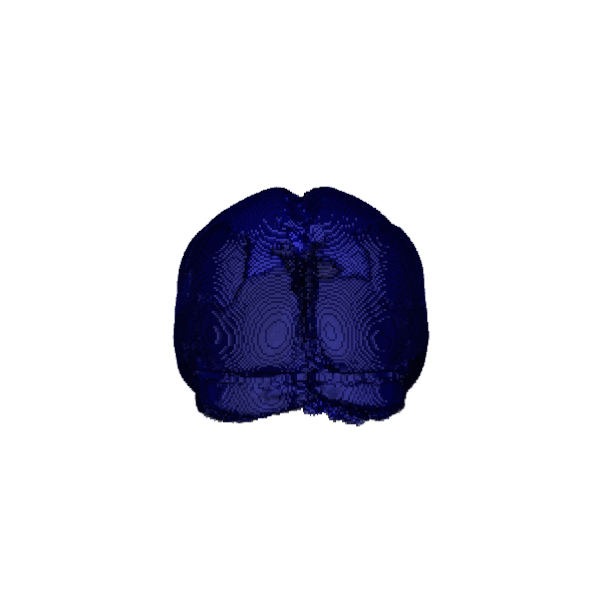
\includegraphics[trim={5cm 5cm  4cm  4cm },clip,height=.3\linewidth]{desikan1a.png}\hspace{-10pt}
  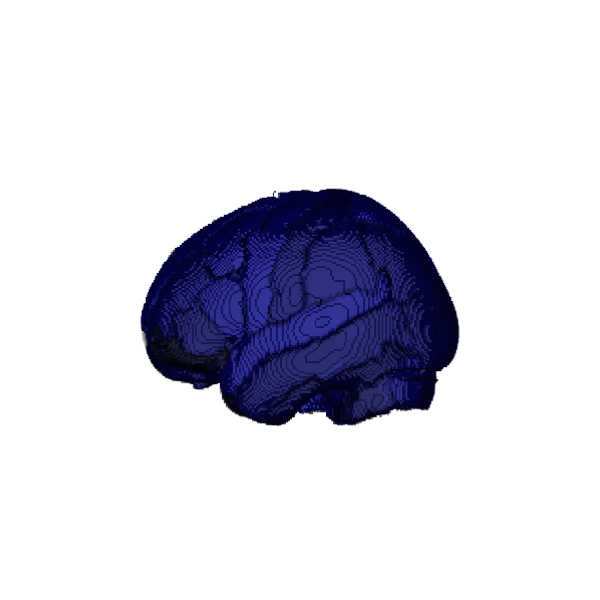
\includegraphics[trim={5cm 5cm  4cm  4cm },clip,height=.3\linewidth]{desikan1b.png}\hspace{-10pt}
  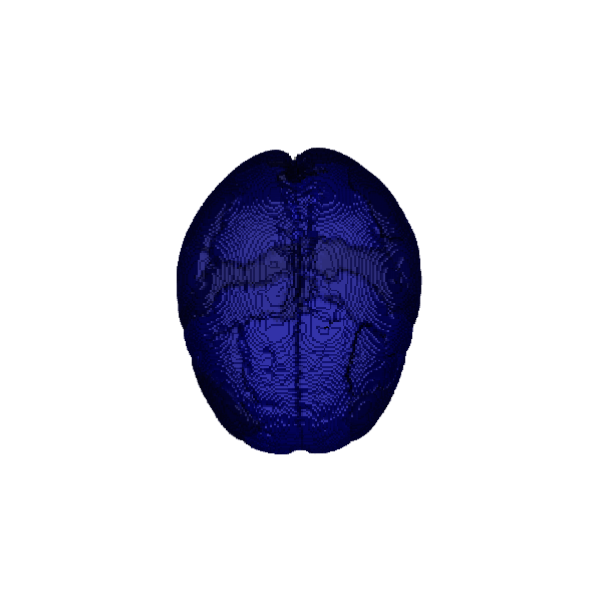
\includegraphics[trim={5cm 5cm  4cm  4cm },clip,height=.3\linewidth]{desikan1c.png}
\end{subfigure}
% \vspace*{5pt}
\begin{subfigure}[t]{0.95\linewidth}
\caption{2nd dimension}
\vspace{-7pt}
\centering
  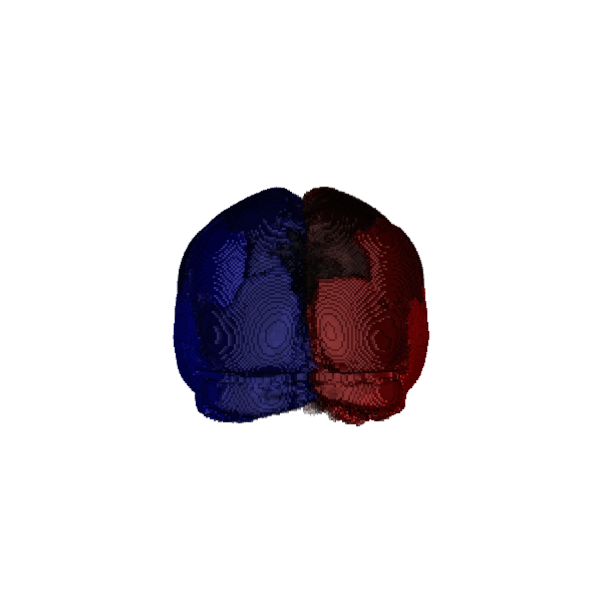
\includegraphics[trim={5cm 5cm  4cm  4cm },clip,height=.3\linewidth]{desikan2a.png}\hspace{-10pt}
  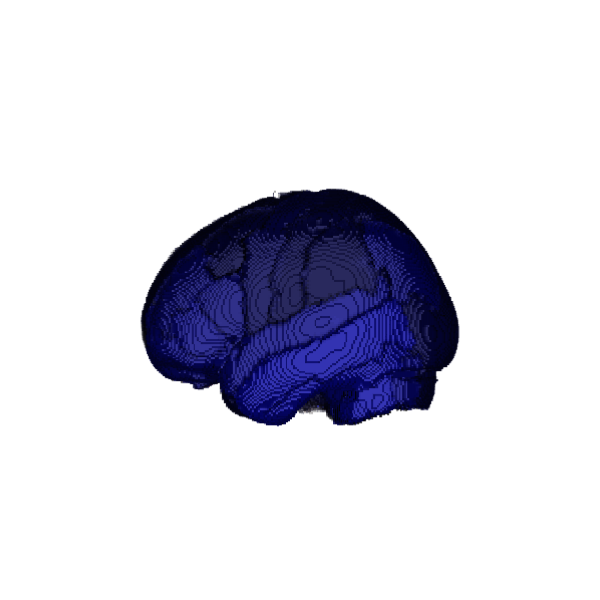
\includegraphics[trim={5cm 5cm  4cm  4cm },clip,height=.3\linewidth]{desikan2b.png}\hspace{-10pt}
  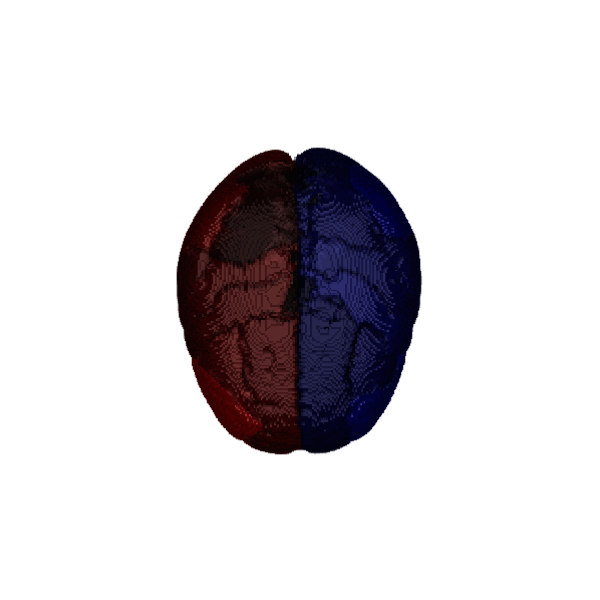
\includegraphics[trim={5cm 5cm  4cm  4cm },clip,height=.3\linewidth]{desikan2c.png}
\end{subfigure}
% \vspace*{5pt}
\begin{subfigure}[t]{0.95\linewidth}
\caption{3rd dimension}
\vspace{-7pt}
\centering
  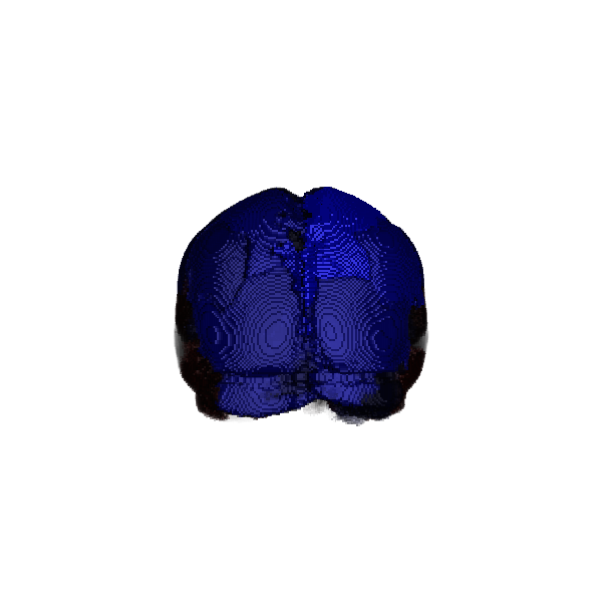
\includegraphics[trim={5cm 5cm  4cm  4cm },clip,height=.3\linewidth]{desikan3a.png}\hspace{-10pt}
  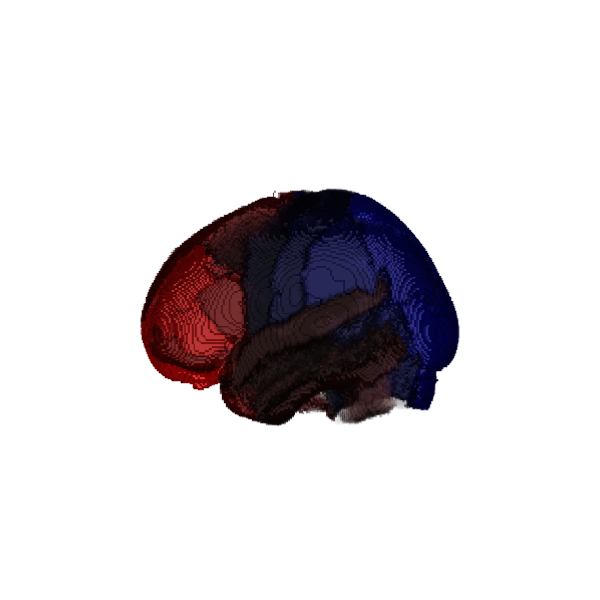
\includegraphics[trim={5cm 5cm  4cm  4cm },clip,height=.3\linewidth]{desikan3b.png}\hspace{-10pt}
  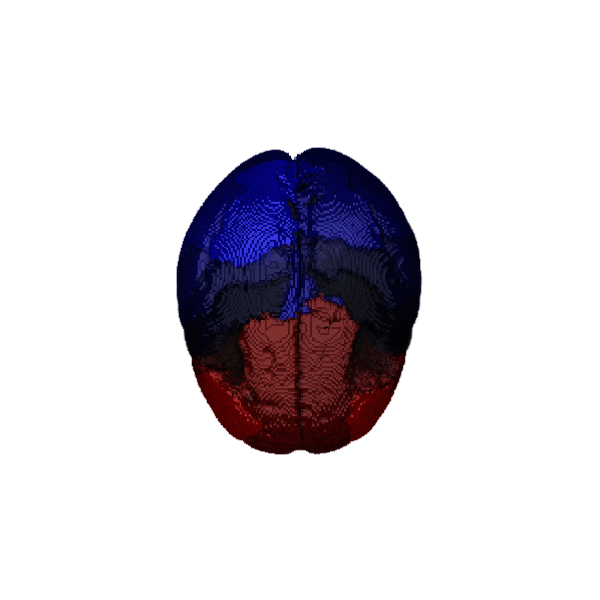
\includegraphics[trim={5cm 5cm  4cm  4cm },clip,height=.3\linewidth]{desikan3c.png}
\end{subfigure}
% \vspace*{5pt}
\begin{subfigure}[t]{0.95\linewidth}
\caption{4th dimension}
\vspace{-7pt}
\centering
  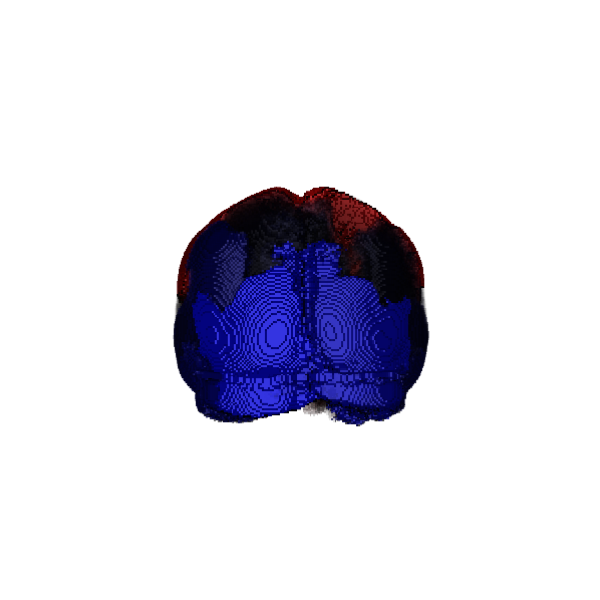
\includegraphics[trim={5cm 5cm  4cm  4cm },clip,height=.3\linewidth]{desikan4a.png}\hspace{-10pt}
  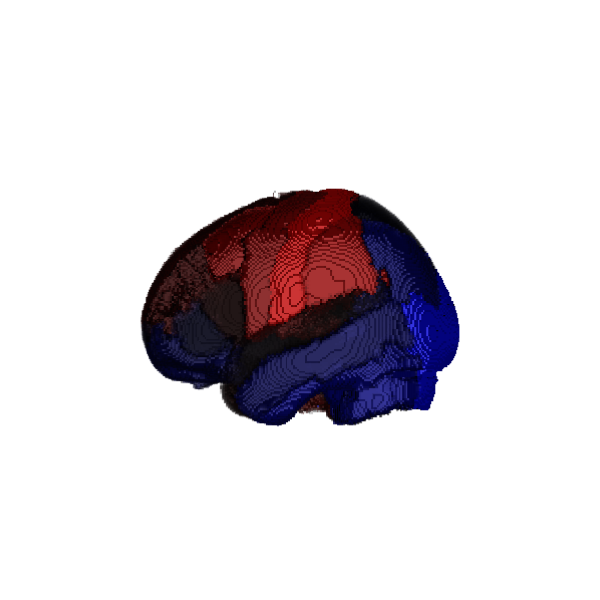
\includegraphics[trim={5cm 5cm  4cm  4cm },clip,height=.3\linewidth]{desikan4b.png}\hspace{-10pt}
  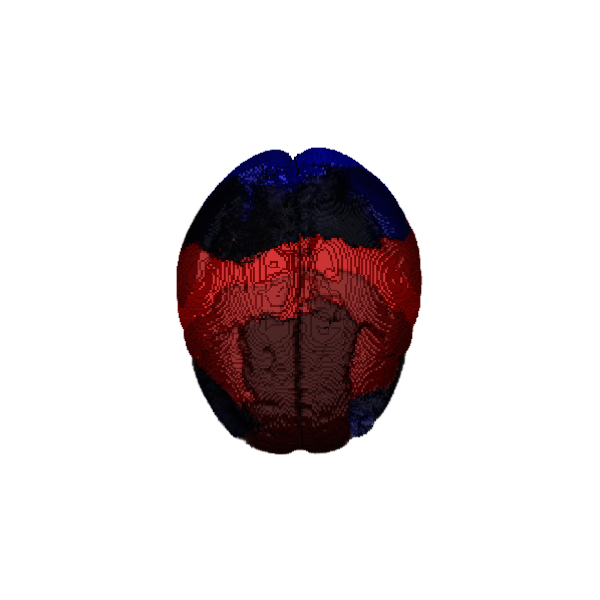
\includegraphics[trim={5cm 5cm  4cm  4cm },clip,height=.3\linewidth]{desikan4c.png}
\end{subfigure}
\caption{
% {\bf Brain plots colored separately for each of the first 4 dimensions of $\hat{X}$ under the Desikan atlas.}
%We color the brain separately for each of the first 5 dimensions of $\hat{X}$.
The color of the $i$-th brain region for the $j$-th dimension is determined by the value of $\hat{X}_{ij}$, i.e.\ the $j$-th element of the estimated latent vector for the $i$-th region. Red represents a positive value while blue represents the negative one, with brighter color indicating larger magnitudes.
The 1st dimension, depicted in Panel (a), is relatively flat across the entire brain. 
In Panel (b), there is a distinction of the left and right hemisphere as conveyed in the 2nd dimension. Similarly, the other dimensions appear to correspond closely with the anatomical lobe structures of the brain (see Section~\ref{section:lobe_structure} for more details).}
\label{fig:eigenvector_brain}
\end{figure}



\subsection{Stochastic Blockmodel as an RDPG}
\label{section:sbm_rdpg}
One of the most common structures for graphs is that vertices tend to cluster into communities where vertices of the same community behave similarly, connecting to similar sets of nodes.
This structural property is captured by the stochastic blockmodel (SBM) \cite{holland1983stochastic}, where each vertex is assigned to a block and the probability that an edge exists between two vertices depends only on their respective block memberships.

% Reviewer 3 mentioned the following references. \cite{ambroise2012new, wolfe2013nonparametric, choi2012stochastic, picard2009deciphering, zanghi2008fast, zanghi2010clustering, pavlovic2014stochastic, daudin2008mixture}.


The SBM is parameterized by the number of blocks $K$ (generally much less than the number of vertices $N$), the block probability matrix $B \in [0,1]^{K \times K}$, and the vector of block memberships
$\tau\in\{1,\dotsc,K\}^N$, where for each $i \in [N]$, $\tau_i = k$ means vertex $i$ is a member of block $k$.

% We will assume each vertex is assigned its block independently according to the probability vector $\rho$, so $\Pr[tau_i = k] = \rho_k$.
Conditioned on $\tau$, each entry of the adjacency matrix $A_{ij}$ ($i < j$) is independently sampled from the Bernoulli distribution with parameter $B_{\tau_i,\tau_j}$.
To ensure that the SBM can be considered as an RDPG, we impose that the $B$ matrix for the SBM is positive semidefinite.
For notational convenience the sub-model of the SBM with positive semidefinite $B$ matrix is referred to  as simply the SBM.

To analyze the estimator $\hat{P}$ motivated by RDPG (Section~\ref{sec:phat} discusses how to construct $\hat{P}$), the SBM can be viewed as an RDPG by
decomposing $B$ as $\nu \nu^{\top}$, where $\nu \in \Re^{K \times d}$ with rows given by $\nu_1^{\top}, \dotsc, \nu_K^{\top}$ and each row $\nu_k^{\top}$ is the shared latent position for all vertices assigned to block $k$.
Let $X \in \Re^{N \times d}$ have rows given by $X_1^{\top} = \nu_{\tau_1}^{\top}, X_2^{\top} = \nu_{\tau_2}^{\top}, \dotsc, X_N^{\top} = \nu_{\tau_N}^{\top}$.
Since $\tau_i$ and $\tau_j$ represent the blocks that vertex $i$ and vertex $j$ belong to respectively:
\[
    \Pr[A_{ij} = 1|\tau] = B_{\tau_i, \tau_j} = \nu_{\tau_i}^{\top} \nu_{\tau_j}^{\phantom{\top}} \in [0, 1].
\]
The SBM is therefore a special case of  an RDPG where all vertices in the same block have identical latent positions.

% An example SBM is illustrated in Fig.~\ref{fig:SBM_example}.
% We consider a 5-block SBM and plot the corresponding probability matrix and one adjacency matrix generated from it with 200 vertices. 
% Panel (a) shows the block-constant structure of the probability matrix and panel (b) shows how this structure is reflected in the random binary adjacency matrix.

% \begin{remark}
% Rather than allowing vertices to differ from each other as in the RDPG, the SBM presumes all nodes within the same block have the same expected degree.
% Vertices in the same block are all stochastically equivalent.
To better describe complex network structures, many
generalizations of the SBM have been explored to incorporate the local variation of vertices to the block structure. 
\cite{airoldi2008mixed} proposed mixed membership stochastic blockmodels, which associates each vertex with multiple blocks with a probability vector rather than a single block as SBM requires.
To model variation of the expected degrees of different vertices within the same block, \cite{karrer2011stochastic} proposed degree-corrected SBM, which assigns additional parameters to each vertex to adjust the expected degree relatively.
These generalizations aim to capture variations among vertices while maintaining aspects of the original community structure.
The RDPG is useful in this regard since any positive semidefinite SBM with degree-correction and mixed membership can be represented as an RDPG and visa versa.
% \end{remark}


\section{Estimators}
\label{sec:estimator}

%In this section, we present two estimators, the standard element-wise sample mean $\bar{A}$, and a low-rank estimator $\hat{P}$.
%We describe the low-rank aspects of this estimator in this section and present further important details regarding diagonal augmentation and dimension estimation in Section~\ref{sec:method}.


% \subsection{Decision Theory}
% % Estimating the mean of a population of samples requires a procedure.
% In statistical decision theory, the risk of a procedure $\delta$ for a given parameter value $\theta\in\Theta$, $R(\delta,\theta)$, is defined as the expected loss. 
% The loss function can be squared Euclidean distance, absolute distance, or other distances \cite{bickel2007mathematical} and the expectation is taken with respect to the given parameter.
% A procedure $\delta^{\prime}$ dominates another procedure $\delta$ if the risk
% of $\delta^{\prime}$ is no bigger than the risk of $\delta$ regardless of the parameter, and strictly less than the risk of $\delta$ in some situations.
% % If there exists a decision procedure $\delta^{\prime}$ which dominates $\delta$, then $\delta$ is said to be inadmissible. So generally, an inadmissible procedure is not preferred since there is another choice which is always ``better'' than it.

% In a striking result, \cite{stein1956inadmissibility} and \cite{james1961estimation} showed that even the arithmetic mean can be dominated by another procedure.
% In particular, James and Stein showed that the sample mean for a multivariate normal distribution with at least three dimensions has strictly higher risk than a procedure that introduces shrinkage, and can be strictly improved by carefully biasing the  estimate towards any given fixed point.
% Twenty-seven years later, \cite{gutmann1982stein} proved that this phenomenon cannot occur when the sample spaces are finite, as is the case for graphs.
% However, while there must be some cases where the sample mean is preferred, this does not imply that other estimators should not be considered.
% In many situations where other structural information is hypothesized, other estimators may be preferable.






% \begin{figure}
% \centering
%   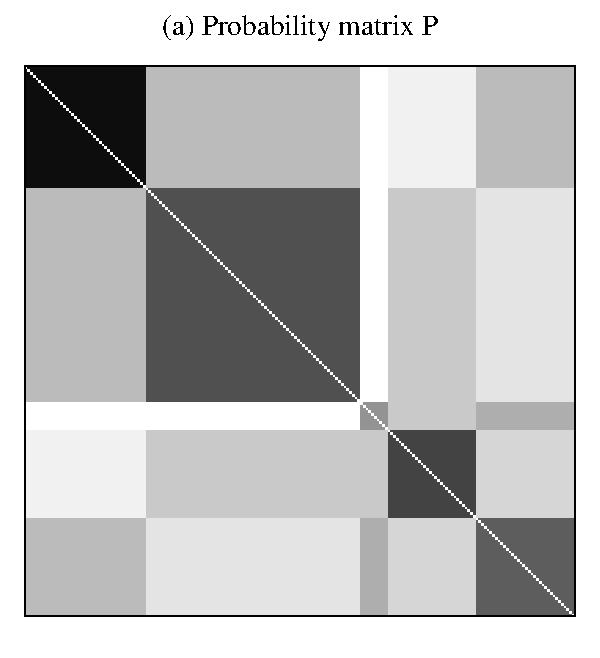
\includegraphics[height=.5\linewidth]{SBM_P.pdf}
%   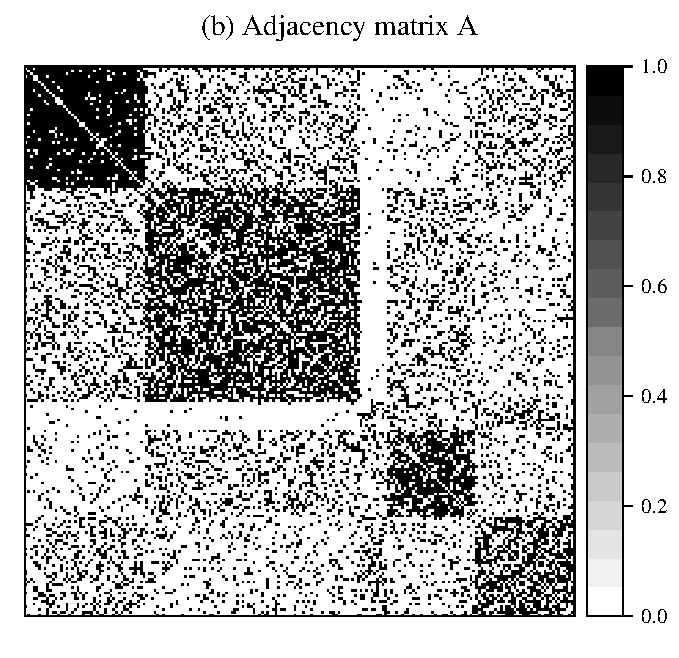
\includegraphics[height=.5\linewidth]{SBM_A.pdf}
%   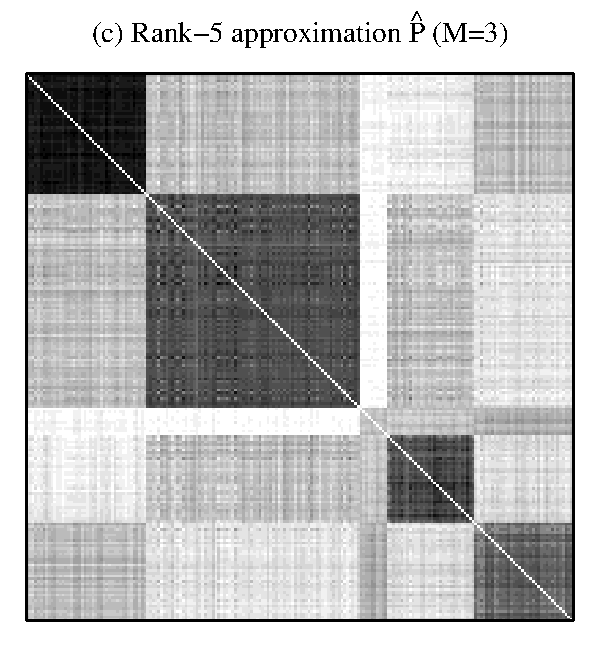
\includegraphics[height=.5\linewidth]{SBM_Phat.pdf}
%   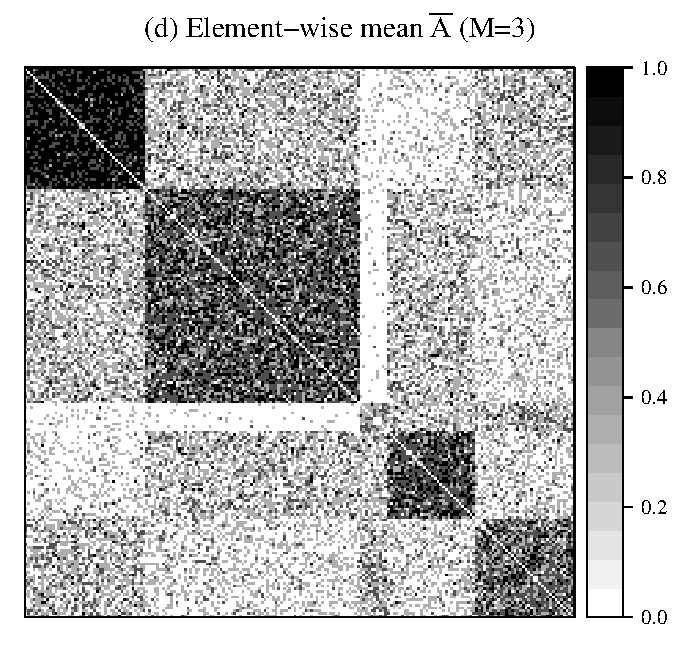
\includegraphics[height=.5\linewidth]{SBM_Abar.pdf}
% \caption{{\bf Stochastic blockmodel example.}
% Panel (a) shows the mean graph $P$ with $K = 5$ blocks and $N=200$ vertices. Panel (b) shows an adjacency matrix $A$ sampled according to the probabilities from $P$.
% While $A$ is a noisy version of $P$, much of the structure of $P$ is preserved in $A$.
% Panel (d) shows the element-wise mean $\bar{A}$
% based on three graphs sampled iid according to the probability matrix $P$.
% Panel (c) shows  our proposed estimate $\hat{P}$, 
% a rank-5 approximation of $\bar{A}$,  thresholding the values to be between $0$ and $1$ (see Section~\ref{sec:phat}).
% Visual inspection shows that the low-rank estimate $\hat{P}$ more closely approximates $P$ as compared to $\bar{A}$.
% Appendix~\ref{section:SBM_parameters} gives all parameters.
% }
% \label{fig:SBM_example}
% \end{figure}


\subsection[Element-wise Sample Mean]{Element-wise Sample Mean $\bm{\bar{A}}$}
\label{sec:abar}

The most natural estimator to consider is the element-wise sample mean.
This estimator, defined as $\bar{A}=\frac{1}{M}\sum_{m=1}^M A^{(m)}$, is the  maximum likelihood estimator (MLE) for the mean graph $P$ if the graphs are sampled from an IEM distribution.
It is unbiased so $\Ex[\bar{A}]=P$ with entry-wise variance $\mathrm{Var}(\bar{A}_{ij}) = P_{ij} (1-P_{ij})/M$. 
Moreover, for the independent edge model, $\bar{A}$ is the uniformly minimum-variance unbiased estimator, so it has the smallest variance among all unbiased estimators.
Similarly, it enjoys the many asymptotic properties of the MLE as $M\to \infty$ for fixed $N$.
However, if graphs with a large number of vertices are of interest, $\bar{A}$ is not consistent for $P$ as the number of vertices $N$ becomes large for fixed $M$, while our estimator $\hat{P}$ discussed in Section~\ref{sec:phat} is consistent for low-rank $P$.
% @rt: "no useful asymptotic properties" is a strong claim.  do we really mean that? do you mean to say that we could not find any in the literature?
% @ds: revised
% @ds2rt: I think maybe you can be specific here. Ie $\bar{A}_{ij}$ does not converge in for this regime but $\hat{P}_{ij}$ does ...
% revised

Additionally, $\bar{A}$ does not exploit any low-dimensional structure.
If the graphs are distributed according to an RDPG or SBM, then $\bar{A}$ is no longer the maximum likelihood estimator since it is not guaranteed to satisfy the properties of the mean graph for that model.
The performance can be especially poor when the sample size $M$ is small, such as when $M\ll N$.
For example, when $M=1$, $\bar{A}$ is simply the binary adjacency matrix $A^{(1)}$, which is an inaccurate estimate for an arbitrary $P$ compared to estimates which exploit underlying structure, such as the low-rank structure of the RDPG model.

\subsection[Low-Rank Estimator]{Low-Rank Estimator $\bm{\hat{P}}$}
\label{sec:phat}

Motivated by the low-rank structure of the RDPG mean matrix, we propose the estimator $\hat{P}$ based on the spectral decomposition of $\bar{A}$ which yields a low rank approximation of $\bar{A}$.
% This estimator does not estimate the parameters of a stochastic blockmodel, as we wish to allow for the increased flexibility of the RDPG.
% However this can be implemented as a step towards estimating SBM parameters.
% 
This estimator is similar to the estimator proposed by \cite{chatterjee2015matrix} but incorporates additional adjustments which serve to improve the performance for the specific task of estimating the mean graph.
Additionally, we consider an alternative dimension selection technique.
Details of the dimension selection procedures and the diagonal augmentation are in Section~\ref{section:dim_select} and \ref{section:diag_aug}, respectively.
To summarize, the overall strategy to compute $\hat{P}$ is described in Algorithm \ref{algo:basic}.
A key component of this algorithm is the low-rank approximation (see Algorithm \ref{algo:lowrank} for details).

The first step is to calculate the sample mean $\bar{A}$.
In Step 2 to Step 4, the algorithm augments the diagonal of $\bar{A}$ based on \cite{marchette2011vertex}, selects the dimension $\hat{d}$ to embed (see Section~\ref{section:dim_select}), and computes the low-rank approximation $\tilde{P}^{(0)}$ based on the embedding. 
Then in Step 5 and Step 6, the algorithm augments the diagonal again based on \cite{scheinerman2010modeling} (see Section~\ref{section:diag_aug}) which yields an improved low-rank estimate $\tilde{P}^{(1)}$.
Finally, Step 7 thresholds the matrix entries to ensure all elements are between 0 and 1.

\begin{algorithm}
\caption{Algorithm to compute $\hat{P}$}
\label{algo:basic}
\begin{algorithmic}[1]
\REQUIRE Adjacency matrices $A^{(1)}, A^{(2)}, \cdots, A^{(M)}$, with each $A^{(m)} \in \{0,1\}^{N \times N}$
\ENSURE Estimate $\hat{P}\in[0,1]^{N\times N}$
\STATE $\bar{A} \leftarrow \left(\sum\limits_{m = 1}^M A^{(m)}\right)/M$;
% @rt: i'd write the equation, and then in comments say that this is the sample mean
\STATE $D^{(0)} \leftarrow \mathrm{diag}(\bar{A} \bm{1})/(N-1)$;
\STATE $\hat{d} \leftarrow \mathrm{dimselect}(\bar{A} + D^{(0)})$; (see Section~\ref{section:dim_select})
% @rt: rather than "select" i'd write ""\hat{d} \leftarrow dimselect(A+D)", or some such
\STATE $\tilde{P}^{(0)} \leftarrow \mathrm{lowrank}_{\hat{d}}(\bar{A} + D^{(0)})$; (see Algorithm~\ref{algo:lowrank})
\STATE $D^{(1)} \leftarrow \mathrm{diag}(\tilde{P}^{(0)})$;
% @rt: i don't quite understand the utility of the above 2 steps
\STATE $\tilde{P}^{(1)} \leftarrow \mathrm{lowrank}_{\hat{d}}(\bar{A} + D^{(1)})$; (see Algorithm~\ref{algo:lowrank})
\STATE $\hat{P} \leftarrow \min(\max(\tilde{P}^{(1)}, 0), 1)$.
% @rt: i don't think i'd use so many words, let "Set to", why not "=" or \leftarrow?
\end{algorithmic}
\end{algorithm}

% @ds: I revised the algorithm and added a description as above.

% \begin{algorithm}[H]
% \caption{Algorithm to compute $\hat{P}$}
% % @rt: perhaps note that this algorithm is parameter free?
% \label{algo:basic}
% \begin{algorithmic}[1]
% \REQUIRE Adjacency matrices $A^{(1)}, A^{(2)}, \cdots, A^{(M)}$, with each $A^{(m)} \in \{0,1\}^{N \times N}$
% \ENSURE Estimate $\hat{P}\in[0,1]^{N\times N}$
% \STATE Calculate the sample mean $\bar{A} = \frac{1}{M}\sum\limits_{m = 1}^M A^{(m)}$;
% % @rt: i'd write the equation, and then in comments say that this is the sample mean
% \STATE Calculate the scaled degree matrix $D^{(0)} = \mathrm{diag}(\bar{A} \bm{1})/(N-1)$;
% \STATE Select the dimension $d$ based on the eigenvalues of $\bar{A} + D^{(0)}$; (see Section~\ref{section:dim_select})
% % @rt: rather than "select" i'd write ""\hat{d} \leftarrow dimselect(A+D)", or some such
% \STATE Set $\tilde{P}^{(0)}$ to $\mathrm{l
% \STATE Set $D^{(1)}$ to $ \mathrm{diag}(\tilde{P}^{(0)})$, the diagonal matrix with diagonal matching $\tilde{P}^{(0)}$;
% % @rt: i don't quite understand the utility of the above 2 steps
% \STATE Set $\tilde{P}^{(1)}$ to s$\mathrm{lowrank}_d(\bar{A} + D^{(1)})$; (see Algorithm~\ref{algo:lowrank})
% \STATE Set $\hat{P}$ to $\tilde{P}^{(1)}$ with values $<0$ set to $0$ and values $>1$ set to $1$.
% % @rt: i don't think i'd use so many words, let "Set to", why not "=" or \leftarrow?
% \end{algorithmic}
% \end{algorithm}


For a given dimension $d$ we consider the estimator $\mathrm{lowrank}_d(\bar{A})$ defined as the best rank-$d$ positive-semidefinite approximation of $\bar{A}$.
Let $\hat{S}$ be a diagonal matrix with non-increasing entries along the diagonal corresponding to the largest $d$ eigenvalues of $\bar{A}$ and let $\hat{U}$ have columns given by the corresponding eigenvectors. Similarly, let $\tilde{S}$ be the diagonal matrix with non-increasing entries along the diagonal corresponding to the rest $N - d$ eigenvalues of $\bar{A}$ and let $\tilde{U}$ have columns given by the corresponding eigenvectors.
Since the graphs are symmetric, the eigen-decomposition can be computed as $\bar{A}$ as $\hat{U} \hat{S} \hat{U}^{\top} + \tilde{U}\tilde{S}\tilde{U}^{\top}=[\hat{U}|\tilde{U}] (\hat{S}\oplus \tilde{S}) [\hat{U}|\tilde{U}]^T$.
The $d$-dimensional adjacency spectral embedding (ASE) of $\bar{A}$ is given by $\hat{X}=\hat{U} \hat{S}^{1/2}\in \Re^{N \times d}$.
For an RDPG, the rows of $\hat{X}$ are estimates of the latent vectors for each vertex \cite{sussman2014consistent}.
Using the adjacency spectral embedding, the low-rank approximation is $\bar{A}$ to be $\hat{X} \hat{X}^{\top}=\hat{U}\hat{S}\hat{U}^{\top}$.
Algorithm~\ref{algo:lowrank} in the appendix gives the steps to compute this low-rank approximation for a general symmetric matrix $A$.

% \begin{algorithm}[H]
% \caption{Algorithm to compute the rank-$d$ approximation of a matrix.}
% \label{algo:lowrank}
% \begin{algorithmic}[1]
% \REQUIRE Symmetric matrix $A\in \Re^{N\times N}$ and dimension $d\leq N$.
% \ENSURE $\mathrm{lowrank}_d(A)\in \Re^{N\times N}$
% \STATE Compute the algebraically largest $d$ eigenvalues of $A$, $s_1\geq s_2\geq \dotsc\geq s_d$ and corresponding unit-norm eigenvectors $u_1,u_2,\dotsc,u_d\in \Re^N$;
% % @rt: this pseudocode is also surprisingly wordy.  i'd write it more formally, with comments.  see, for example, the pseudocodes at the end of my MGC paper with cencheng
% \STATE Set $\hat{S}$ to the $d\times d$ diagonal matrix $\mathrm{diag}(s_1,\dotsc,s_d)$;
% \STATE Set $\hat{U} = [u_1,\dotsc,u_d]\in \Re^{N\times d}$;
% \STATE Set $\mathrm{lowrank}_d(A)$ to $\hat{U}\hat{S}\hat{U}^{\top}$;
% \end{algorithmic}
% \end{algorithm}

To compute the estimator $\hat{P}$, the rank $d$  must be specified; there are various ways of dealing with dimension selection.
In this paper, we explore an elbow selection method proposed in \cite{zhu2006automatic} and the universal singular value thresholding (USVT) method \cite{chatterjee2015matrix}.
Section~\ref{section:dim_select} discusses details of these methods.

Moreover, since the adjacency matrices are hollow, with zeros along the diagonal, there is a missing data problem that leads to inaccuracies if $\hat{P}$ is computed based only on $\bar{A}$.
To compensate for this issue, we use an iterative method developed in \cite{scheinerman2010modeling}.
Section~\ref{section:diag_aug} discusses details of the iterative method.





% Algorithm~\ref{algo:basic} gives the steps involved to compute the low-rank estimate $\hat{P}$.
% The bottom panels of Fig.~\ref{fig:SBM_example} demonstrate the two estimators $\hat{P}$ and $\bar{A}$ for the stochastic blockmodel given by Panel (a).
% The estimates are based on a sample of size $M=3$ and in this instance visual inspection demonstrates that $\hat{P}$ performs much better than $\bar{A}$.
% As  in the succeeding sections, this procedure will frequently yield improvements in estimation as compared to using the sample mean $\bar{A}$.
% While this is not surprising for random dot product graphs, where we are able to show theoretical results to this effect, we also see this effect for connectome data and more general independent edge graphs.
% In the following sections, this estimator is explored in the context of the stochastic blockmodel.



% \section{Statistical Efficiency}
% \label{sec:result}


\section{Theoretical Results}
\label{section:theoretical_result}
To estimate the mean of a collection of graphs, we consider the two estimators from Section~\ref{sec:estimator}: the entry-wise sample mean $\bar{A}$ and the low-rank $\hat{P}$ motivated by the RDPG.
The mean squared errors (MSE) for our estimators are $\mathrm{MSE}(\hat{P}_{ij})=\Ex[\hat{P}_{ij}-P]^2$ and $\mathrm{MSE}(\bar{A})=\Ex[\bar{A}_{ij}-P]^2$.
% While one can directly compare the difference in mean squared errors between the two estimators, it is frequently useful to consider the relative efficiency between two estimators.
The relative efficiency for two estimators is the ratio of their MSE, $\mathrm{RE}(\bar{A}_{ij},\hat{P}_{ij}) = \frac{\mathrm{MSE}(\hat{P}_{ij})}{\mathrm{MSE}(\bar{A}_{ij})}$, with values above 1 indicating $\bar{A}$ should be preferred while values below 1 indicate $\hat{P}$ should be preferred.
Relative efficiency is a useful metric for comparing estimators because it will frequently be invariant to the scale of the noise in the problem and hence is comparable across different settings.

In this section, entry-wise relative efficiency is computed to analyze the performance of these two estimators under the SBM.
The asymptotic relative efficiency is defined as $\lim_{N\to \infty}\mathrm{RE}$.
%, with the number of graphs $M$ fixed.
We also define the scaled relative efficiency, $N\cdot \mathrm{RE}(\bar{A}_{ij},\hat{P}_{ij})$ which normalizes the relative efficiency so that the asymptotic scaled relative efficiency is non-zero and finite.
Somewhat surprisingly, the results indicate that the asymptotic relative efficiency will not depend on this fixed sample size $M$.


For this asymptotic framework, we assume the block memberships $\tau_i$ are drawn iid from a categorical distribution with block membership probabilities given by $\rho\in[0,1]^K$.
In particular, this implies that for each block $k$, the proportion of vertices in block $k$, $|\{i:\tau_i=k\}|/N$, will converge to $\rho_k$ as $N\to\infty$ by the law of large numbers.
We will also assume that for a given $N$, the block membership probabilities are fixed for all graphs.
Denote the block probability matrix as $B = \nu \nu^{\top} \in [0, 1]^{K \times K}$.
By definition, the mean of the collection of graphs generated from this SBM is $P \in [0, 1]^{N \times N}$, where $P_{ij} = B_{\tau_i, \tau_j}$. After observing $M$ graphs on $N$ vertices $A^{(1)}, \cdots, A^{(M)}$ sampled independently from the SBM conditioned on $\tau$, the two estimators can be calculated, $\bar{A}$ and $\hat{P}$.

\begin{lemma}
\label{lm:VarPhat}
For the above setting, for any $i \ne j$, if $\mathrm{rank}(B)=K=d$; for large enough $N$,
\[
    \Ex[(\hat{P}_{ij} - P_{ij})^2] \approx
    \frac{1/\rho_{\tau_i} + 1/\rho_{\tau_j}}{M N} P_{ij}(1-P_{ij}),
\]
and
\[
    \lim_{N \to \infty} N \cdot \mathrm{Var}(\hat{P}_{ij}) =
    \frac{1/\rho_{\tau_i} + 1/\rho_{\tau_j}}{M} P_{ij} (1 - P_{ij}).
\]
\end{lemma}


\begin{theorem}
\label{thm:ARE}
In the same setting as in Lemma~\ref{lm:VarPhat}, for any $i \ne j$, if $\mathrm{rank}(B)=K=d$, then for large enough $N$:
\begin{equation}
	    \mathrm{RE}(\bar{A}_{ij}, \hat{P}_{ij}) \approx
    \frac{1/\rho_{\tau_i} + 1/\rho_{\tau_j}}{N}.
\label{eq:approx_re}
\end{equation}
And the asymptotic relative efficiency (ARE) is
\[
    \mathrm{ARE}(\bar{A}_{ij}, \hat{P}_{ij}) = \lim_{N \to \infty} \mathrm{RE}(\bar{A}_{ij}, \hat{P}_{ij}) = 0.
    \label{eq:sbm_are}
\]
\end{theorem}

% The first part of this lemma ensures that the estimator is asymptotically unbiased for $P$,
% and the second part gives the form of the asymptotic variance of $\hat{P}$.
Note that $\rho_{\tau_i}$ represents the probability that a vertex is assigned to the same block as vertex $i$, i.e.\ $\tau_i$-th block.
The proofs of these results are provided in Section~\ref{section:outline_proof}. 
% and is based on results for the variance of the adjacency spectral embedding from \cite{athreya2016limit}.  
% Lemma \ref{lm:VarPhat} shows that the MSE of $\hat{P}_{ij}$ has order $O(M^{-1}N^{-1})$ in terms of $M$ and $N$, regardless of the SBM parameters. Similar to $\bar{A}$, the estimate will get better as the number of observations $M$ increases.
However, it also benefits from more vertices since the number of parameters for a low-rank $P$ grows slowly compared to the number of potential edges as the number of vertices increases. That is, $\hat{P}$ will perform better as the number of vertices $N$ increases.

% Moreover, since $\bar{A}_{ij}$ is the sample mean of $M$ independent Bernoulli random variables with parameter $P_{ij}$, then
% \[
    % \Ex[(\bar{A}_{ij} - P_{ij})^2] = \frac{P_{ij}(1-P_{ij})}{M}.
% \]
% Based on this MSE result of $\bar{A}_{ij}$ and the MSE result of $\hat{P}_{ij}$ given by Lemma \ref{lm:VarPhat}, the next theorem follows.




This theorem indicates that under the SBM, $\hat{P}$ is a much better estimate of the mean of the collection of graphs $P$ than $\bar{A}$, especially when $N$ is large.
Note that a relative efficiency less than 1 indicates that $\hat{P}$ should be preferred over $\bar{A}$, so under the above assumptions, as $N\to\infty$, $\hat{P}$ performs far better than $\bar{A}$.
Note that even though the RE could be greater than $1$ for some $N$, eventually the RE will go to 0 as $N$ increases.
The result shows that the relative efficiency is of order $O(N^{-1})$ and $N \cdot \mathrm{RE}(\bar{A}_{ij}, \hat{P}_{ij})$ (which is denoted as scaled RE) converges to $1/\rho_{\tau_i}+1/\rho_{\tau_j}$ when $N\to\infty$.
An important aspect of Theorem~\ref{thm:ARE} is that the ARE does not depend on the number of graphs $M$, so the larger the graphs are, the better $\hat{P}$ is relative to $\bar{A}$, regardless of $M$.
% @rt: we say as N \to \infty a bunch in the above.  when N "equals" infinity, RE is 1.  perhaps worth clarifying explicitly in the above that while RE >1 as n increases, eventually, RE=1?
% @ds: revised

The asymptotic results are for a number of vertices going to infinity with a fixed number of graphs, a setting which will be very useful in future connectomics analysis, as the collection of larger and larger brain networks grow from small sample sizes.
 % as the technology to scale these connectome collection techniques is developed.
For example, \cite{Calabrese2015} recently reported a high resolution magnetic resonance microscopy based estimate of the mouse brain using a single mouse.
% The above paragrph could use another sentence to link the connectome of the single mouse brain to a larger sample size in the future. -Toni

The approximate formula Eq.~\ref{eq:approx_re} indicates that the sizes of the blocks can greatly impact the relative efficiency.
As an example, consider a 2-block SBM.
If each of the blocks contain half the vertices, then for each pair of vertices, the relative efficiency is approximately $4/N$.
If the first block gets larger, with $\rho_1\to 1$, then the RE for estimating $P_{ij}$ with $\tau_i=\tau_j=1$ will tend to its minimum of $2/N$.
On the other hand as $\rho_1\to 1$, if $\tau_i=1$ and $\tau_j=2$, then, since $\rho_2=1-\rho_1$, the relative efficiency for estimating such an edge pair will be approximately $1$ and the same will hold if $\tau_i=\tau_j=2$.
Note that the maximum value for the relative efficiency of two vertices from different blocks in a two-block model is achieved when $\rho_1=1/N$ and $\rho_2=(N-1)/N$ in which case the relative efficiency is $N/(N-1) \approx 1$.
(Values of $\rho_s$ below $1/N$ correspond to graphs where no vertices are typically in that block, so the effective minimum that can be considered for $\rho_s$ is $1/N$.)
Note, $N \cdot \mathrm{RE}(\bar{A}_{ij}, \hat{P}_{ij})$ achieves its minimum for $i$ and $j$ from different blocks when $\rho_k = 1/K$ for all $k$.

Finite sample simulations illustrating these results are in Sec.~\ref{sec:sbm_sim}.
% , which corresponds to $\rho_1=\rho_2=1/2$ in the 2-block case.

% If for example there is one block containing half the vertices, the relative efficiency for estimating the probabilities of edges between vertices in that block will be approximately $4/N$.
% For even larger blocks, the relative efficiency will decrease towards $1/N$ as the proportion of the verties in that block tends.
% If a block has very few vertices, the asymptotic relative efficiency will tend towards one, but will always be less than one.
% x



% \begin{figure}[!t]
% \centering
% 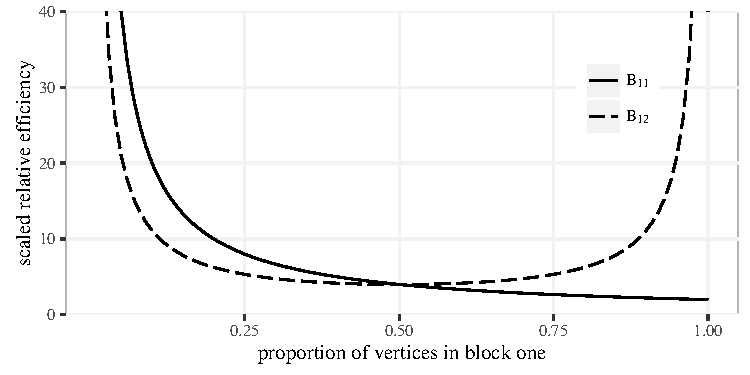
\includegraphics[width=1\linewidth]{rho.pdf}
% \caption{{\bf Asymptotic scaled relative efficiency $N\cdot \mathrm{RE}(\bar{A},\hat{P})$ in a 2-block SBM.}
% For each two distinct pairs of edge probabilities in a 2-block SBM, the scaled relative efficiency only depends on the proportion of vertices in each block.
% As $\rho_1$ changes from $0,1$, the scaled ARE is shown for pairs of vertices where either both are in block one, $B_{11}$, or one is in block one and one is in block two, $B_{12}$.
% These curves intersect at a scaled relative efficiency of 4 when $\rho_1=1/2=\rho_2$.
% Improvements using low-rank methods are greater for larger blocks, such as for $B_{11}$ when $\rho_1$ is near 1, while the improvements are smaller for block pairs with relatively few vertex pairs such as $B_{11}$ when $\rho_1$ is small and $B_{12}$ when $\rho_1$ is near 0 or 1
% .
% Note that the curve for $B_{22}$ would be the same as that for $B_{11}$ but reflected around the vertical line when $\rho_1=1/2$.
% % Simulated results for scaled RE, i.e. $N \cdot \mathrm{RE}_{st}(\bar{A}, \hat{P})$ with $N = 500$ and $M = 100$ of 1000 Monte Carlo replicates while changing $\rho_1$ from 0.1 to 0.9. Scaled relative efficiency in average with different $N$ and fixed $M$ based on 1000 Monte Carlo replicates. Different types of lines denote the simulated values associated with the edges we are averaging over. Notice that when $\rho_1 = 0.5$, the scaled RE has value $4.0$, which agrees with the result in Fig~\ref{fig:RE} as expected.}
% Overall, $\hat{P}$ performs best for large blocks while the improvements may be very minor for blocks with only a few vertices.
% }
% \label{fig:RErho}
% \end{figure}



% % To illustrate Eq.~\ref{eq:approx_re} of Theorem~\ref{thm:ARE}, we consider a 2-block SBM with parameters
% % \begin{equation}
% % B = \begin{bmatrix}
% % 0.42 & 0.2 \\
% % 0.2 & 0.7
% % \end{bmatrix}
% % ,\qquad \rho = \begin{bmatrix}
% % 0.5 & 0.5
% % \end{bmatrix},
% % \label{eq:sim_setting}
% % \end{equation}
% % so that $|\{i:\tau_i=1\}| \approx |\{i:\tau_i=2\}|$, especially for large $N$.
% % Note that this simulation only focuses on the rank-2 setting primarily for the interpretability.
% % When calculating $\hat{P}$, we omit the dimension selection step from Algorithm~\ref{algo:basic} and instead use the true dimension $d = \mathrm{rank}(B) = 2$.
% Fig.~\ref{fig:RErho} shows curves for $2/\rho_1$ and $1/\rho_1+1/\rho_2$ i, the scaled asymptotic RE for pairs of vertices both in block one and pairs of vertices in different blocks, respectively, in terms of $\rho_1$.
% We vary $\rho_1$ between 0 and 1 to demonstrate how the number of pairs of vertices with the corresponding block memberships impacts the overall relative efficiency.
% % For $N=500$ and $M=100$, estimates of the scaled RE $N \cdot \mathrm{RE}(\bar{A}_{ij}, \hat{P}_{ij})$ based on simulations agree very closely with their corresponding theoretical values displayed in the figure. Note that when $\rho_1 = 0.5$, the scaled RE has value $4.0$, which agrees with the result in Fig.~\ref{fig:RE} for simulated data.

% @rt: perhaps worth pointing out that the min N*RE = 1, and it is only that bad when rho_i = 1/K for all i?
% @ds: revised


If instead of assuming that the graphs follow an SBM distribution, we assume that the graphs are distributed according to an RDPG distribution, similar gains in relative efficiency can be realized.
While there is no compact analytical formula for the relative efficiency of $\hat{P}$ versus $\bar{A}$ in the general RDPG case, using the same ideas as in Theorem~\ref{thm:ARE}, we can show that $\mathrm{RE}(\bar{A}_{ij},\hat{P}_{ij}) = O(1/N)$.

\begin{proposition}
Suppose that $A^{(1)},A^{(2)},\dotsc,A^{(M)}$ are independently and identically distributed from an RDPG distribution with common latent positions $X_1,\dotsc,X_n$, which are drawn iid from a fixed distribution.
As the number of vertices $N\to\infty$, it holds for any $i\neq j$ that $\mathrm{RE}(\bar{A}_{ij},\hat{P}_{ij}) = O(1/N)$,
where again the asymptotic relative efficiency in $N$ does not depend on $M$.
\end{proposition}
The proof of this proposition closely follows the proofs of Lemma~\ref{lm:VarPhat} and Theorem~\ref{thm:ARE}.
% , and hence it is omitted here.

\begin{remark}\label{remark:low_rank}
As noted above, if the graphs are distributed according to an SBM or an RDPG, the relative efficiency is approximately invariant to the number of graphs $M$ when $N$ is large.
If on the other hand, the graphs are generated according to a full-rank independent edge model, then the relative efficiency can change more dramatically as $M$ changes.
For larger $M$, more of the eigenvectors of $\bar{A}$ will begin to concentrate around the eigenvectors of the mean graph.
This leads to the fact that the optimal embedding dimension for estimating the mean will increase, making $\bar{A}$ and the optimal low-rank approximation more similar.
As a result, $\mathrm{RE}(\bar{A},\hat{P})$ will increase as $M$ increases for full-rank models, wit $\mathrm{RE}(\bar{A},\hat{P})$ possibly $\geq 1$ since it is not guaranteed that $\hat{P}$ will choose the optimal dimension.
% The lack of gaps in the eigenvalues of the mean graph makes dimension reduction quite dangerous.
% In an extreme case, the low-rank assumption will be most violated when all eigenvalues of the mean graph are almost equal. This leads to a certain type of structure, which is close to a constant times the identity matrix. However, such structure is not seen in connectomics.
This will be discussed further in Section \ref{sec:corr_data} when applying the estimator to the SWU4 dataset.
\end{remark}

\section{Connectomics}\label{sec:connectome}

\subsection{Human Connectomes}\label{sec:corr_data}
In practice, observed graphs do not follow the independent edge model, let alone an RDPG or SBM, but the mean of a collection of graphs is still of interest for these cases.
To demonstrate that the estimator $\hat{P}$ is still useful in such cases, its performance on structural connectomic data was tested.
The graphs are based on diffusion tensor MR images of SWU4 dataset collected and available at the Consortium for Reliability and Reproducibility (CoRR) \cite{zuo2014open} (see Section~\ref{section:data_human}).
The dataset contains 454 different brain scans, each of which was processed to yield an undirected, unweighted graph with no self-loops, using the pipeline described in \cite{kiar2017science, kiar2016ndmg}.
The vertices of the graphs represent different regions in the brain defined according to an atlas.
Here, three atlases were used: the JHU atlas with 48 vertices \cite{oishi2010mri}, the Desikan atlas with 70 vertices \cite{desikan2006automated}, and the  CPAC200 atlas with 200 vertices \cite{sikka2014towards}.
An edge exists between two vertices whenever there is at least one white-matter tract connecting the corresponding two regions of the brain.
Further details of the dataset are provided in Section~\ref{section:data}.

%As discussed in Remark \ref{remark:low_rank}, we first check if the dataset has the low-rank property. In Fig.~\ref{fig:screeplot}, we plot the eigenvalues of the mean graph of all 454 graphs (with diagonal augmentation) in decreasing algebraic order for three different atlases. For all three atlases, the eigenvalues first decrease dramatically and then stay around 0. In addition, we also plot the histograms in Fig.~\ref{fig:histogram}. From the figures we can see many eigenvalues are around zero, with a few large eigenvalues. So the information is mostly contained in the first few dimensions. Such quasi low-rank property could be used by $\hat{P}$ to improve $\bar{A}$.

%\begin{figure}[!htbp]
%\centering
%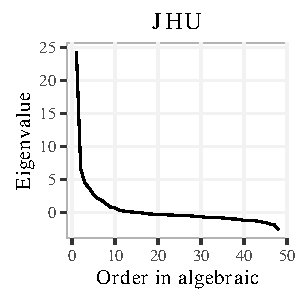
\includegraphics[height=.2\textheight]{screeplot_JHU.pdf}
%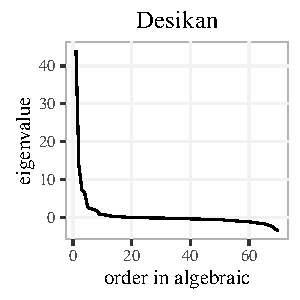
\includegraphics[height=.2\textheight]{screeplot_desikan.pdf}
%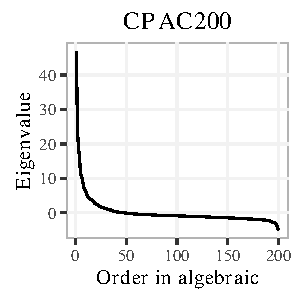
\includegraphics[height=.2\textheight]{screeplot_CPAC200.pdf}
%\caption{{\bf Screeplot of the population mean.}
%These screeplots show the eigenvalues of the mean graph of all 454 graphs with diagonal augmentation in decreasing algebraic order for three atlases. Many eigenvalues are around zero, which lead to a quasi low-rank structure.
%}
%\label{fig:screeplot}
%\end{figure}

% \subsecti on{Estimating Mean Connectomes from Diffusion MRI Data}

A cross validation on the 454 graphs of each size evaluated the performance of the two estimators.
Specifically, for a given atlas, each Monte Carlo replicate corresponds to sampling $M$ graphs out of the 454 and computing the low-rank estimator $\hat{P}$ and the sample mean $\bar{A}$ using the $M$ selected graphs.
These estimates were compared to the sample mean for the remaining $454-M$ adjacency matrices.
While we cannot interpret this mean graph as the probability matrix for an IEM distribution (see Section~\ref{sec:sim_iem}), the sample mean for the remaining graphs does give the proportion of times each pair of vertices are adjacent in the population from  the sampled graphs.

% While in previous sections the mean squared error for either an individual entry or for an entire block in the SBM were evaluated, in this section and the next section we will focus on the overall error for estimating the mean graph.

To evaluate performance, the ratios of the average of the mean squared error across all vertex pairs is computed.
 % of vertices, in conjunction with $\mathrm{MSE}(\bar{A})$ and $\mathrm{MSE}(\hat{P})$ will determine the relative efficiency, where $\mathrm{MSE}(\bar{A})$ is defined as $\mathrm{MSE}(\bar{A}) = \binom{N}{2}^{-1} \sum_{i<j}\Ex[(\bar{A}_{ij}-P_{ij})^2]$ and $\mathrm{MSE}(\hat{P})$ is similarly defined.
% As in the previous section, analytical evaluations of the MSE will not be evaluated, and instead estimates of the MSE and relative efficiencies via from Monte Carlo simulations will be employed.
% By observing 454 graphs generated by the atlas being picked, we use $\hat{P}$ to estimate the mean graph $P$, which is the proportions of the existence of a white-matter tract connecting different parts of the brain. Since $P$ is unknown in practice, we perform a cross-validation study to compare $\bar{A}$ and $\hat{P}$. For each Monte Carlo replicate, we first fix the sample size $M$ and randomly sample $M$ graphs from the total 454 graphs in the dataset. We assure $M$ to be relatively small such that the entry-wise mean of the remaining $(454 - M)$ graphs is a valid approximation of the true probability matrix $P$ we are estimating. Then we can calculate $\bar{A}$ and $\hat{P}$ based on the $M$ samples and compare their performance based on the estimated probability matrix.
1000 cross-validation simulations on each of the three atlases were run for sample sizes of $M=1, 5, 10$. For $M=1$, only the 454 distinct possibilities were considered.
To determine the rank for $\hat{P}$, we employed Zhu and Ghodsi's method \cite{zhu2006automatic} and USVT \cite{chatterjee2015matrix}.
Section~\ref{section:dim_select} discusses details of these methods.



\begin{figure}
\begin{center}
  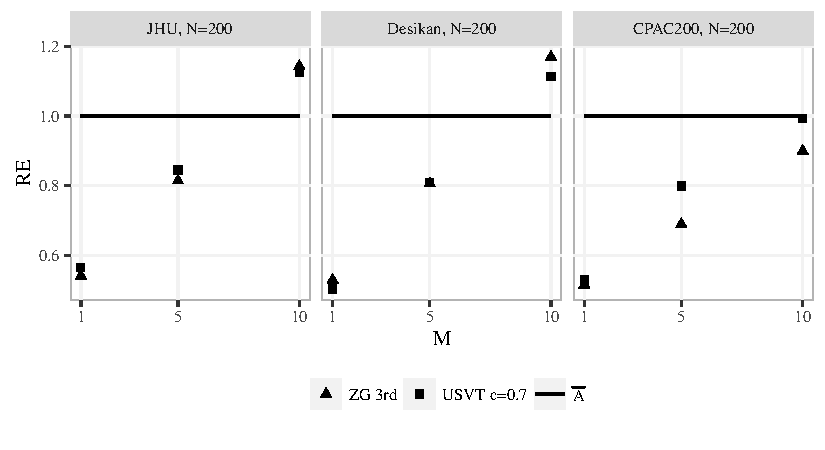
\includegraphics[width=1\linewidth]{corr_data_REdiff.pdf}
\end{center}
\caption{
% {\bf Relative efficiencies of $\bar{A}$ versus $\hat{P}$ for the SWU4 data set.}
A sampling of graphs from each atlas: JHU, Desikan, and CPAC 200, had $\bar{A}$ and $\hat{P}$ computed using different sample sizes $M$ and different dimension selection procedures, ZG and USVT.
For each of the two methods for computing $\hat{P}$, relative efficiencies were estimated with respect to the sample mean $\bar{A}$.
Confidence intervals all had lengths less than $0.015$, and hence were omitted for clarity.
% The largest improvements using $\hat{P}$ occur when $M$ is small and $N$ is large, where the RE are smaller than 1.
% On the other hand, once $M=10$, $\bar{A}$ tends to do nearly as well or better than $\hat{P}$.
% Overall, the relative efficiencies are greater for smaller sample sizes $M$ and larger number of vertices $N$.
}
\label{fig:corr_re}
\end{figure}

Fig.~\ref{fig:corr_re} shows the estimated relative efficiencies between $\bar{A}$ and $\hat{P}$.
For each atlas and each sample size, both dimension selection methods have similar overall performance.
Confidence intervals for the estimated relative efficiencies, calculated by assuming a normal distribution, all have lengths less than $0.015$.
Hence, except for the CPAC200 atlas with $M=10$, all relative efficiencies are significantly different from 1.

The largest improvements using $\hat{P}$ occur when $M$ is small and $N$ is large, where the RE are smaller than 1.
On the other hand, once $M=10$, $\bar{A}$ tends to do nearly as well or better than $\hat{P}$.
% In addition, $\hat{P}$ offers certain advantages, especially since low-rank estimates can often be more easily interpretable by considering the latent position representation described in Section~\ref{section:sbm_rdpg}.

% As discussed in Section~\ref{sec:intro}, Fig.~\ref{fig:Matrix_desikan_m5}  further illustrates the differences between the two estimators for a samples with size $M=5$ and $M=1$.
% For the sample with $M=5$, $\hat{P}$ was calculated using  Zhu and Ghodsi's 3rd elbow to select $d=11$.
% As discussed above, $\hat{P}$ has a finer gradient of estimated probabilities and has fewer outliers than $\bar{A}$, as shown in the upper triangular part of panels (b) and (e).


For the sample with size $M=5$ illustrated in Fig.~\ref{fig:Matrix_desikan_m5}, Fig.~\ref{fig:Diff_desikan_m5} shows the values for the absolute estimation error $|\bar{A} - P|$ and $|\hat{P}-P|$, as well as $|\bar{A} - \hat{P}|$.
The lower triangular sections show the actual absolute difference while the upper triangular matrix highlights vertex pairs with absolute differences larger than 0.4.
There are 18 edges for $\bar{A}$ and only 6 edges for $\hat{P}$ being highlighted in the figure.
Note that approximately $13\%$ of all pairs of vertices are adjacent in all $454$ graphs and hence $\bar{A}$ will always have zero error for those pairs of vertices.
Nonetheless, $\hat{P}$ typically outperforms $\bar{A}$.

\begin{figure}
\begin{center}
  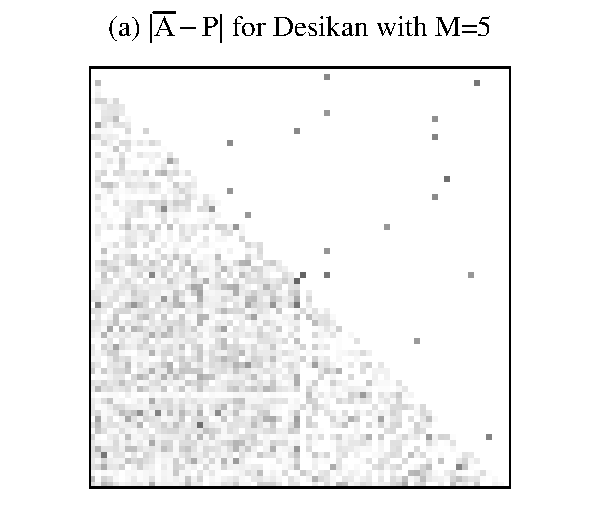
\includegraphics[height=.325\linewidth]{Diff2_desikan_m5.pdf}\hspace{-35pt}
  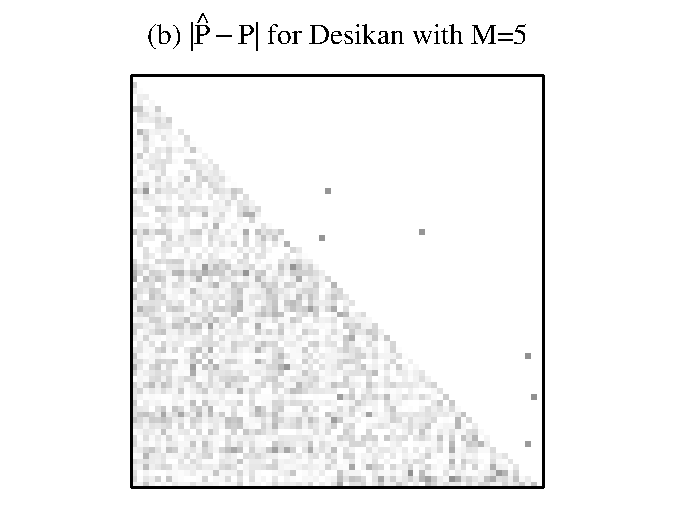
\includegraphics[height=.325\linewidth]{Diff3_desikan_m5.pdf}\hspace{-28pt}
  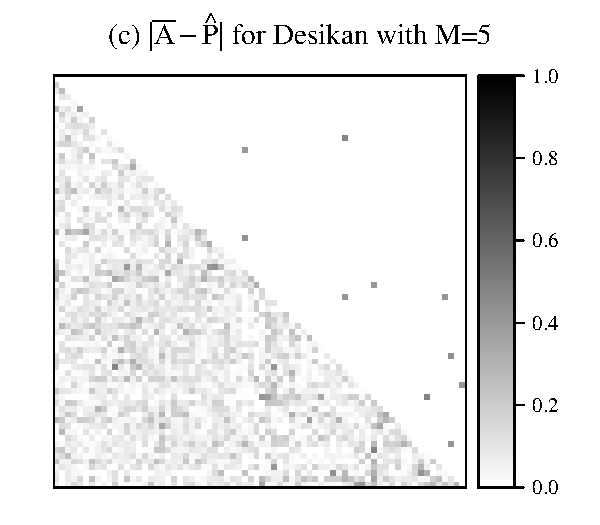
\includegraphics[height=.325\linewidth]{Diff1_desikan_m5.pdf}
\end{center}
\caption{
% {\bf Heat plots of absolute estimation.}
The lower triangular matrices show the absolute estimation error $|\bar{A} - P|$, $|\hat{P} - P|$ and $|\bar{A} - \hat{P}|$ for a sample of size $M=5$ from the Desikan dataset.
The embedding dimension for $\hat{P}$ is $d=11$ selected by the ZG method. 
The upper triangular matrix highlights the edges with absolute differences larger than $0.4$, with 18 edges from $\bar{A}$ and only 6 edges from $\hat{P}$ being highlighted.
}
\label{fig:Diff_desikan_m5}
\end{figure}

In Fig.~\ref{fig:Diff_between_desikan} we plot the 50 edges with the largest differences $|\bar{A}_{ij} - P_{ij}| - |\hat{P}_{ij} - P_{ij}|$ according to the location of the corresponding regions in the brain. Red edges indicate that $\hat{P}$ overestimates $P$, while blue means that $\hat{P}$ underestimates $P$. The edge width is determined by the estimation error for $\hat{P}$, where pairs with larger estimation error are represented by thicker lines.
The five regions corresponding to vertices that contribute most to the difference are also highlighted, which are the vertices $i$ with the largest value of $\sum_j (|\bar{A}_{ij} - P_{ij}| - |\hat{P}_{ij} - P_{ij}|)$.

Three of these top five regions form a contiguous group of regions.
The top five regions are the inferior temporal, middle temporal, and transverse temporal regions in the left hemisphere and the parahippocampal and pars opercularis regions in the right hemisphere of the Desikan atlas.
The regions that differ most appear to be predominantly localized to the temporal lobe, where increased regionally-specific noise in the diffusion weighted imagining data may increase the estimation error.

\begin{figure}[!htbp]
\centering
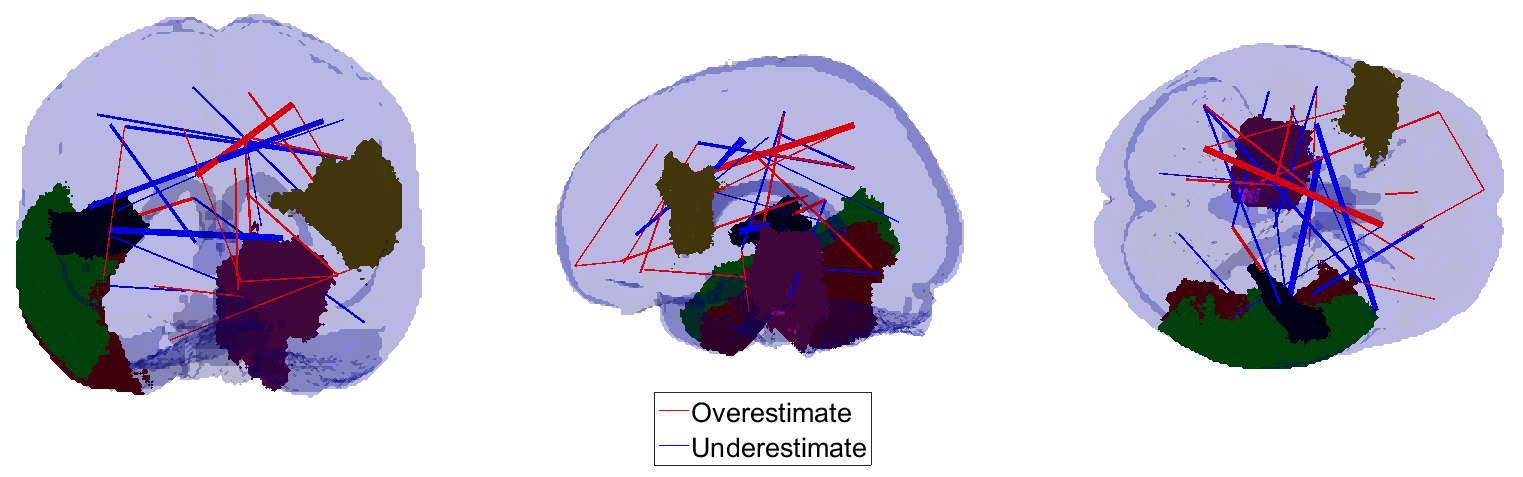
\includegraphics[width=1\linewidth]{Diff_Between_desikan.png}
\caption{ Top 5 regions of the brain and top 50 connections between regions with the largest differences $\bm{|\bar{A}_{ij} - P_{ij}| - |\hat{P}_{ij} - P_{ij}|}$.
Red edges indicate that $\hat{P}$ overestimates $P$ while blue means that $\hat{P}$ underestimates $P$. The edge width is determined by the estimation error. 
% Connections with larger estimation error are represented by thicker lines. This figure shows the regions and connections of the brain where $\hat{P}$ outperforms $\bar{A}$ the most for estimating $P$.
}
\label{fig:Diff_between_desikan}
\end{figure}

\subsection{Challenges of the SWU4 Dataset}
\label{sec:challenge}

While our estimator $\hat{P}$ performs well when the sample size $M$ is small and the number of vertices $N$ is large, the CoRR dataset itself does not strictly adhere to the low-rank assumptions of our theory.
%Unlike simulations, for real data, we can never know the true population mean graph $P$ that we are trying to estimate based on a finite observations. However, in order to compare different estimators, we are going to use the entry-wise sample mean of all 454 graphs as the true but unknown mean graph $P$, which is preferable to $\bar{A}$ compared to $\hat{P}$. From now on, if not specified particularly, when we say $P$ it means the entry-wise sample mean of the 454 graphs.
As discussed in Remark \ref{remark:low_rank}, whether the dataset has low-rank structure was first investigated. In Fig.~\ref{fig:screeplot}, the relative error $\|\mathrm{lowrank}_d(P)-P\|_F^2/\|P\|_F^2$ of using a rank-$d$ approximation of $P$ (see Algorithm~\ref{algo:lowrank}) is plotted as solid curves.
The rate at which this curve tends to zero provides an indication of the relative performance of using $\hat{P}_d$ as compared to $\bar{A}$ when $M$ is large.
For all three atlases, substantial errors remain for any low-rank approximation.
This can be compared to the dashed lines which show how these errors would behave if $P$ was truly low-rank where the ranks are selected by Zhu and Ghodsi's method, 13 for JHU, 8 for Desikan, and 37 for CPAC200.
% @rt: truly what rank? rank 10?
% @ds: I add that they are selected by ZG
% @ds2rt: Give the specific number!
% revised. 13/8/37
% As can be expected, 
% As it turns out, the SWU4 dataset is not even approximately low-rank.
% , which violates the low-rank assumption.

%Since we are using the entry-wise sample mean graph of 454 observations as $P$, it is possible that the true but unknown population mean has the low-rank property but the entry-wise sample mean graph fails to capture it. And it is also possible that the population mean $P$ is actually high-rank. No matter which one is true, the low-rank assumption is violated, which makes this real data experiment setting preferable to the entry-wise sample mean $\bar{A}$ compared to the low-rank estimator $\hat{P}$.

\begin{figure}[!htbp]
\centering
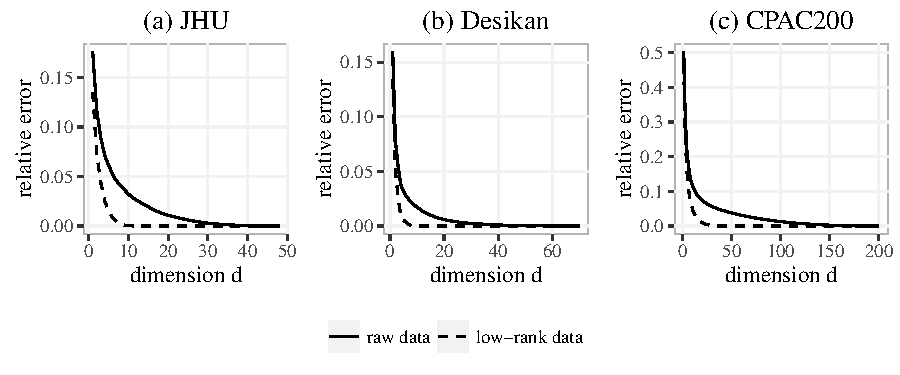
\includegraphics[width=\linewidth]{screeplot_ratio_all.pdf}
\caption{
% {\bf Relative error of the rank-$d$ approximation of the population mean.}
The solid curves show the relative error $\|\mathrm{lowrank}_d(P)-P\|_F^2/\|P\|_F^2$ of using a rank-$d$ approximation of $P$ (see Algorithm~\ref{algo:lowrank}) for three different atlases.
The relative error decays relatively slowly when $d$ is close to $N$, which indicates that $P$ is not low-rank.
For a $P$ which is actually low-rank, the relative error is plotted with the dashed curves.}
\label{fig:screeplot}
\end{figure}

%\begin{figure}[!htbp]
%\centering
%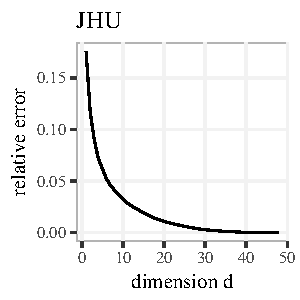
\includegraphics[height=.2\textheight]{screeplot_ratio_JHU.pdf}
%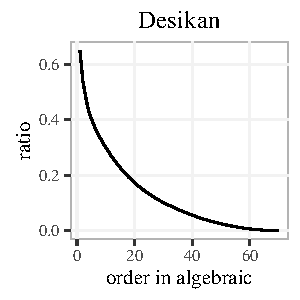
\includegraphics[height=.2\textheight]{screeplot_ratio_desikan.pdf}
%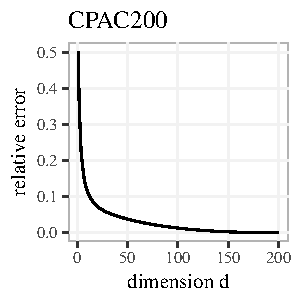
\includegraphics[height=.2\textheight]{screeplot_ratio_CPAC200.pdf}
%\caption{{\bf Relative error of the rank-$d$ approximation of the population mean.}
%These plots show the relative error $\|\mathrm{lowrank}_d(P)-P\|_F^2/\|P\|_F^2$ of using a rank-$d$ approximation of $P$ (see Algorithm~\ref{algo:lowrank}) for three different atlases.
%The relative error
%The relative error decays relatively slowly is large unless $d$ is close to $N$, which indicates that $P$ is not low-rank.
%In particular note }
%\label{fig:screeplot}
%\end{figure}

%\begin{figure}[!htbp]
%\centering
%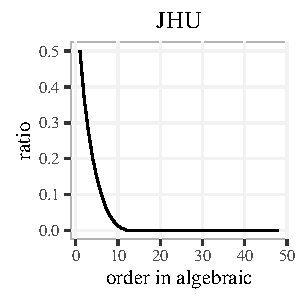
\includegraphics[height=.2\textheight]{screeplot_ratio_JHU_lowrank.pdf}
%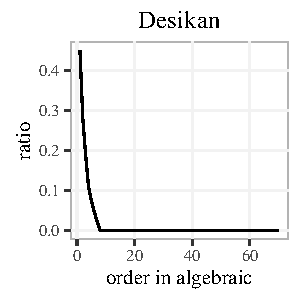
\includegraphics[height=.2\textheight]{screeplot_ratio_desikan_lowrank.pdf}
%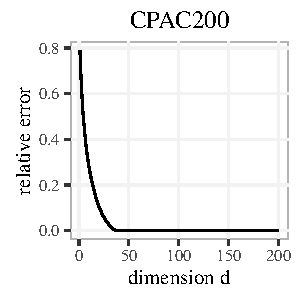
\includegraphics[height=.2\textheight]{screeplot_ratio_CPAC200_lowrank.pdf}
%\caption{{\bf Relative error of the rank-$d$ approximation of the low-rank population mean.}
%For all three atlases, we revise $P$ to be low-rank by only keeping a few large eigenvalues. The dimensions we keep are selected by the Zhu and Ghodis method.
%These plots show the relative error of using a rank-$d$ approximation of the revised $P$ for three different atlases.}
%\label{fig:screeplot_lowrank}
%\end{figure}

% In addition, by plotting the histograms of the eigenvalues of $P$ in Fig.~\ref{fig:histogram}, we see that there are a bunch of negative eigenvalues, which indicates that the positive semi-definiteness is also violated in this real data experiment. This makes it even harder for $\hat{P}$ to outperform $\bar{A}$.

% \begin{figure}[!htbp]
% \centering
% 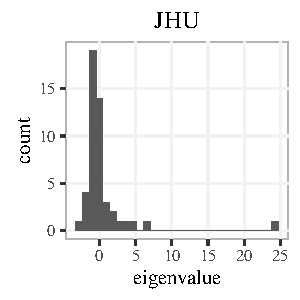
\includegraphics[height=.2\textheight]{hist_JHU.pdf}
% 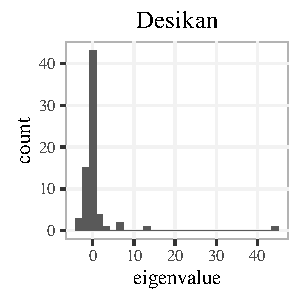
\includegraphics[height=.2\textheight]{hist_desikan.pdf}
% 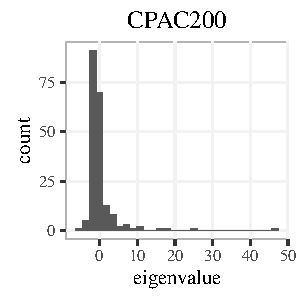
\includegraphics[height=.2\textheight]{hist_CPAC200.pdf}
% \caption{{\bf Histogram of the population mean.}
% These figures show the histograms of the eigenvalues of the mean graph of all 454 graphs with diagonal augmentation. A bunch of negative eigenvalues indicate that $P$ is not positive semi-definite.
% }
% \label{fig:histogram}
% \end{figure}

This dataset has other challenges for low-rank methods.
First, there are a large number of negative eigenvalues which $\hat{P}$ will not capture.
Low-rank methods can be made to include large negative eigenvalues, however, for low sample sizes excluding negative eigenvalues improved performance.
Second, approximately 12.8\% of the entries of $P$ are exactly equal to 1.
For these edges, $\bar{A}$ will have exactly zero error, while $\hat{P}$ will be a less accurate estimate.


% Moreover, by the histogram of $P$, i.e. the entry-wise mean of all 454 graphs based on the Desikan atlas, as in Fig.~\ref{fig:P_hist_desikan}, we can clearly see more edge probabilities are concentrated on both sides, i.e. close to 0 or 1. In particular, 12.8\% of the edges has probability equals to 1 exactly. For these edges, MLE $\bar{A}$ always recover the probability 1 exactly even with only 1 observation, while $\hat{P}$ will give a less accurate estimate because of the smoothing effect. So the CoRR dataset we consider is highly preferable to $\bar{A}$ compared to $\hat{P}$.
%However, even in this situation, $\hat{P}$ still outperforms $\bar{A}$ when the sample size is relatively small.

% \begin{figure}[!htbp]
% \centering
% 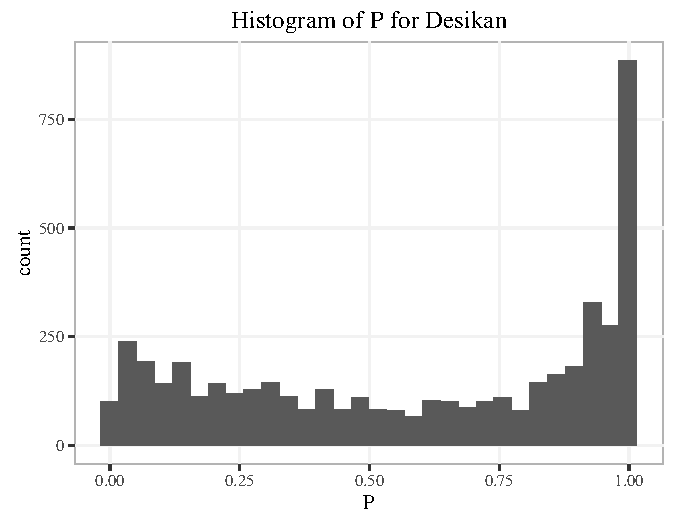
\includegraphics[width=0.8\textwidth]{P_hist_desikan.pdf}
% \caption{{\bf Histogram of $P$ for Desikan atlas.}
% This figure shows the histogram of $P$, i.e. the entry-wise mean of all 454 graphs based on the Desikan atlas. More edge probabilities of $P$ are concentrated on both sides, i.e. close to 0 or 1. In particular, 12.8\% of the edges has probability equals to 1 exactly.}
% \label{fig:P_hist_desikan}
% \end{figure}

Despite these challenges, when the sample size is relatively small, such as $M=1$ or $M=5$, and for larger number of vertices, $\hat{P}$ gives a better estimate than $\bar{A}$ for the CoRR dataset.
(See Appendix~\ref{sec:sim_iem} for a similar synthetic data analysis.)
Importantly, this improvement is robust to the embedding dimension as illustrated in Section~\ref{sec:dim}.
% We should note that though the total error for $\hat{P}$ is smaller in this case, for certain entries $\bar{A}$ does perform better.
% For example, there are some pairs of vertices that are adjacent for all samples in the population and for these pairs $\bar{A}$ will always perform better than $\hat{P}$.



\subsection{Lobe Structure}
\label{section:lobe_structure}
In addition to yielding potentially improved estimation, low-rank methods help provided convenient interpretations simultaneously. 
% In this section, the focus is on how the lobe structure is reflected in the low-rank estimate and the estimated latent positions in particular.

Classically, the brain can be divided into lobes, originally based purely on anatomical considerations, now widely recognized to also play a functional role \cite{Vanderah2015}.
While different anatomists partition brain regions differently, there is general agreement on four cortical lobes per hemisphere: frontal, parietal, occipital, and temporal \cite{fischl2012freesurfer,desikan2006automated,salat2004thinning}.
For the Desikan atlas, there are 70 different regions (35 regions for each hemisphere), with each region belonging to a single lobe (see Appendix~\ref{section:data_human}). 
% Three regions of the Desikan atlas per hemisphere (Banks of Superior Temporal Sulcus, Corpus Callosum, and the ``Unknown'' region) 
% do not have obvious lobe assignment and were clustered into a new lobe category named ``other'' to resolve this issue.

One might expect that properties of regions within a lobe are more similar to those across lobes, even upon conditioning on anatomical proximity, as regions within lobes would be expected to share more functional roles.
To test whether the embedded latent positions $X$ preserve this property or not, we propose a test statistic $T$ to be the average differences between vertices within the same lobe minus the average differences between vertices across different lobes, i.e.

\begin{equation}
	T(X, l) = \sum_{i \ne j} \frac{\mathbf{1}_{l(i) = l(j)}\|X_i - X_j \|_2}{\sum_{k \ne l} \mathbf{1}_{l(k) = l(l)}} -
\frac{ \mathbf{1}_{l(i) \ne l(j)}\|X_i - X_j \|_2}{\sum_{k \ne l} \mathbf{1}_{l(k) \ne l(l)}}, \label{eq:test_stat}
\end{equation}
where $l(i)$ denotes the lobe assignment for vertex $i$.
If the latent positions $X$ and the lobe assignment $l$ are independent, then $T(X, l)$ will be close to zero.
A small test statistic $T(X, l)$ indicates that latent positions of the regions within the same lobe are closer compared to the ones across the lobes.

% To test this hypothesis the lobe labels of each region were randomly permutated and the test statistics calculated $T(X, l^{\prime})$ based on the permuted lobe labels $l^{\prime}$. 
% After performing 1000 Monte Carlo replicates of unconditional permutations, the p-value is less than $10^{-12}$.

However, the anatomical geometry might contribute to the dependence between $X$ and $l$, with spatially proximal vertices having similar connectivity patterns.
% and we do not want to be distracted by this factor. So instead of testing the dependence between $X$ and $l$, we are more interested in the following hypothesis test:
Hence, a small test statistic $T(X, l)$ is evidence that the low-rank methods preserve the lobe structure only if we also condition on anatomy geometry:
$H_0: X$ and $l$ are conditionally independent given anatomical geometry,
$H_A: X$ and $l$ are conditionally dependent given anatomical geometry.
% A test of these hypotheses will focus on how much of the lobe structure is really captured by the latent positions associated with the low-rank methods without being affected by the inherent spatial relationship.
The test of conditional independence has less power compared to the test of unconditional independence which is performed with a random permutation of lobe labels (which yield a p-value $<10^{-6}$).

To test under the anatomical geometry conditions, the lobe assignment $l$ was permuted so that the number of regions in each lobe remain the same and the regions within the same randomly defined lobe are still spatially connected. 
A flip was defined to be a swap of two pairs of vertices which preserves the number of regions in each lobe and also maintains the constraint that lobes are spatially contiguous.
The lobes are flipped a limited number of times in order to study how the number of flips impacts the test statistic.
Appendix~\ref{section:testing} discusses the flipping procedure.

1000 simulations with the test statistics  of $T(X, l')$ are shown for a fixed number of flips after the permutation. 
The number of flips was varied from 1 to 10  (Fig.~\ref{fig:violin_plot}). In the violin plot, the dashed line indicates the value of $T(X, l)$ based on the true lobe assignment. 
% $T(X, l)$ for the true lobe assignment moves away from the the $2.5\%$-quantile based for the random permutations. 
% The figure shows corresponding p-values.
The p-value is less than 0.05 if the number of flips is larger than 7.
Hence, latent positions in the same lobe are more similar to each other, even after accounting for the fact that geometrically proximal regions may also have similar latent positions.
When the number of flips is small, this test has very little power, with the null distribution a small deviation from the original lobes.
 % @rt: i don't understand the above.  "regardless" means not using it in the estimate? please clarify.
% @ds: revised. maybe we can have a better way?
% @ds2rt: I also don't understand. It suggests that latent positions in the same lobe are more similar to each other, even after accounting for the fact that geometrically proximal regions may also have similar latent positions.
% revised

\begin{figure}[!htbp]
\centering
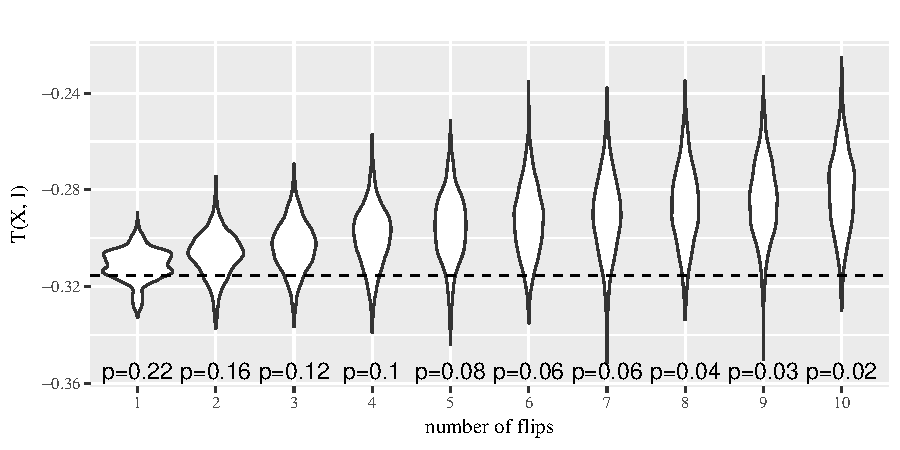
\includegraphics[width=1\linewidth]{violinplot_new_flip_2norm_1_8.pdf}
\caption{
% {\bf Violin plot of the permutation test.}
1000 simulations were run for each number of flips. Dashed line represents the statistic $T(x,l)$ based on true lobe assignment. As the null hypotheses move further from the original lobe assignment, the 95\% central region of the null distributions shifts away from $T(x,l)$ under the true lobe assignment.}
\label{fig:violin_plot}
\end{figure}

%\begin{figure}[!htbp]
%\centering
%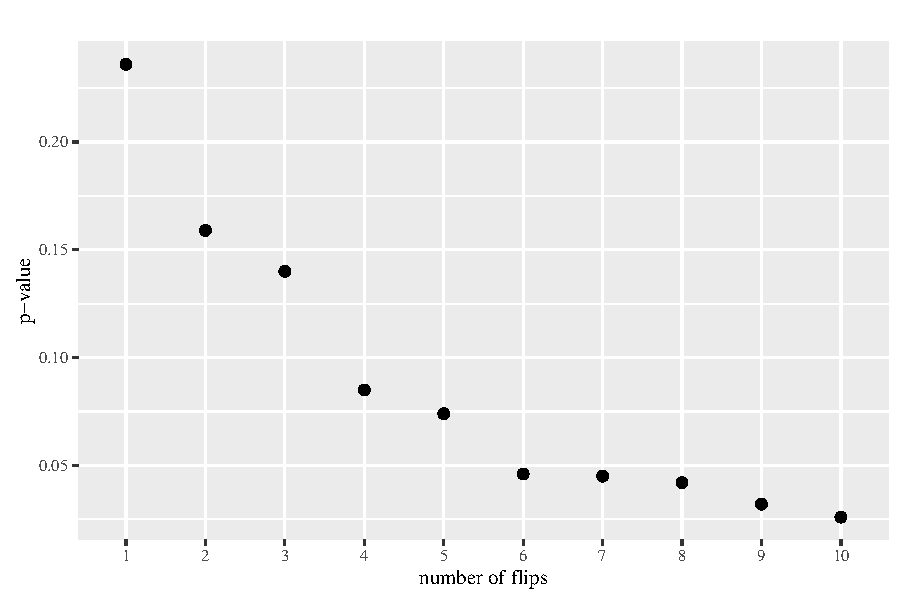
\includegraphics[width=0.8\textwidth]{pvalue_new_flip_2norm_1_8.pdf}
%\caption{{\bf P-value of the permutation test.}
%This figure shows the p-value of the permutation test based on different number of flips. When the number of flips is larger than 7, the p-value is less than 0.5, which suggests that the latent positions based on the low-rank methods preserves the lobe structure.}
%\label{fig:pvalue}
%\end{figure}





%\begin{figure}[!htbp]
%\centering
%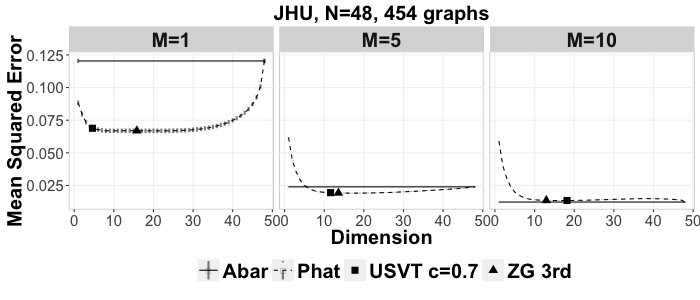
\includegraphics[width=1\textwidth]{JHU.png}
%\caption{Comparison of MSE between $\bar{A}$ (solid line) and $\hat{P}$ (dashed line) for JHU dataset while embedding the graphs into different dimensions with different size $M$ of the subsamples. The dimension chosen by the 3rd elbow of Zhu and Ghodsi is denoted in triangle, and chosen by USVT with threshold equals 0.7 is denoted in square. Vertical intervals represent the 95\% confidence interval. When $M$ is small, $\hat{P}$ outperforms $\bar{A}$ with a flexible range of the embedding dimension including what Zhu and Ghodsi selects.}
%\label{fig:JHU}
%\end{figure}
%
%\begin{figure}[!htbp]
%\centering
%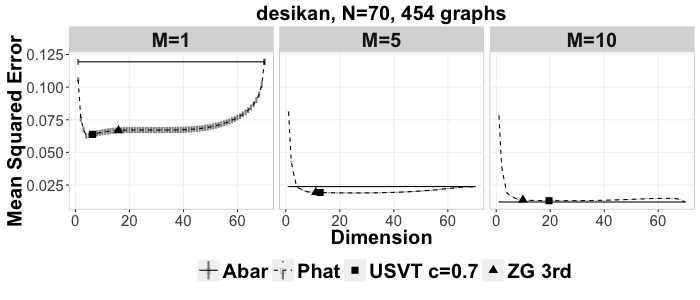
\includegraphics[width=1\textwidth]{desikan.png}
%\caption{Comparison of MSE between $\bar{A}$ (solid line) and $\hat{P}$ (dashed line) for desikan dataset while embedding the graphs into different dimensions with different size $M$ of the subsamples. The dimension chosen by the 3rd elbow of Zhu and Ghodsi is denoted in triangle, and chosen by USVT with threshold equals 0.7 is denoted in square.  Vertical intervals represent the 95\% confidence interval.  When $M$ is small, $\hat{P}$ outperforms $\bar{A}$ with a flexible range of the embedding dimension including what Zhu and Ghodsi selects.}
%\label{fig:desikan}
%\end{figure}
%
%\begin{figure}[!htbp]
%\centering
%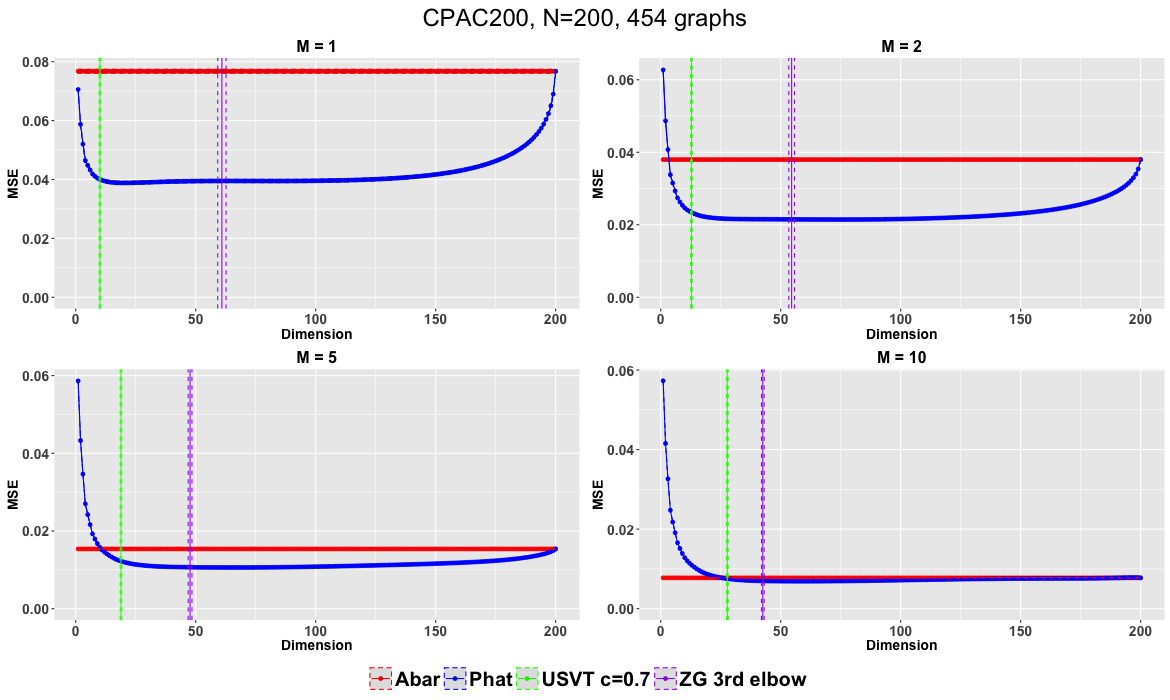
\includegraphics[width=1\textwidth]{CPAC200.png}
%\caption{Comparison of MSE between $\bar{A}$ (solid line) and $\hat{P}$ (dashed line) for CPAC200 dataset while embedding the graphs into different dimensions with different size $M$ of the subsamples. The dimension chosen by the 3rd elbow of Zhu and Ghodsi is denoted in triangle, and chosen by USVT with threshold equals 0.7 is denoted in square.  Vertical intervals represent the 95\% confidence interval.  When $M$ is small, $\hat{P}$ outperforms $\bar{A}$ with a flexible range of the embedding dimension including what Zhu and Ghodsi selects.}
%\label{fig:CPAC200}
%\end{figure}
%
%\begin{figure}
%\centering
%\begin{subfigure}{.33\textwidth}
%  \centering
%  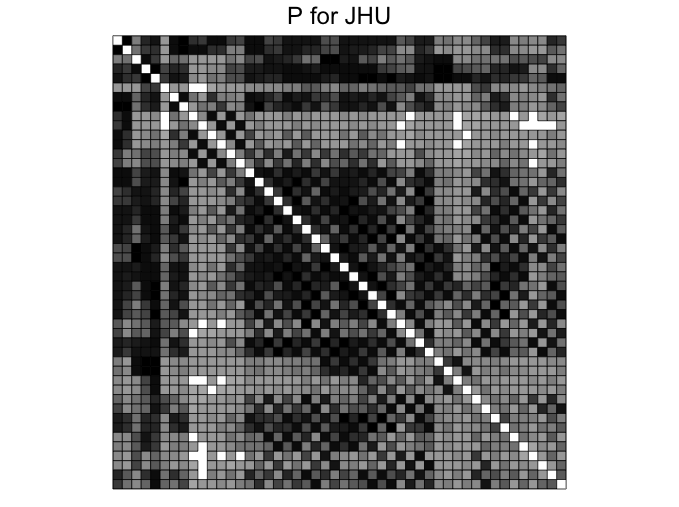
\includegraphics[width=1.2\linewidth]{P_JHU.png}
%\end{subfigure}%
%\begin{subfigure}{.33\textwidth}
%  \centering
%  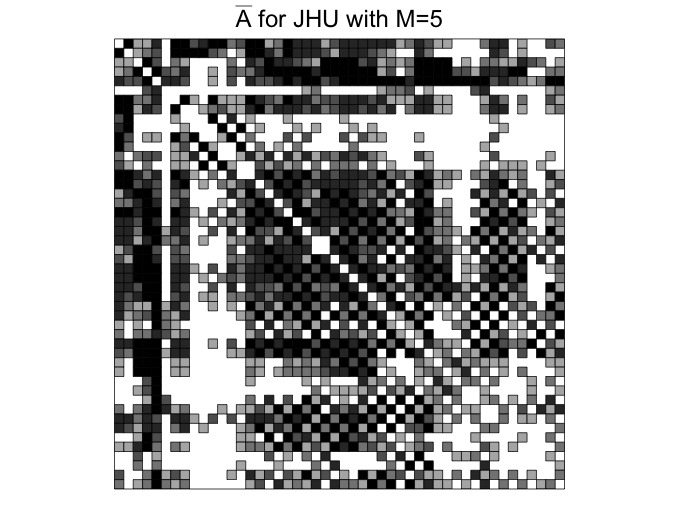
\includegraphics[width=1.2\linewidth]{Abar_JHU_m5.png}
%\end{subfigure}
%\begin{subfigure}{.33\textwidth}
%  \centering
%  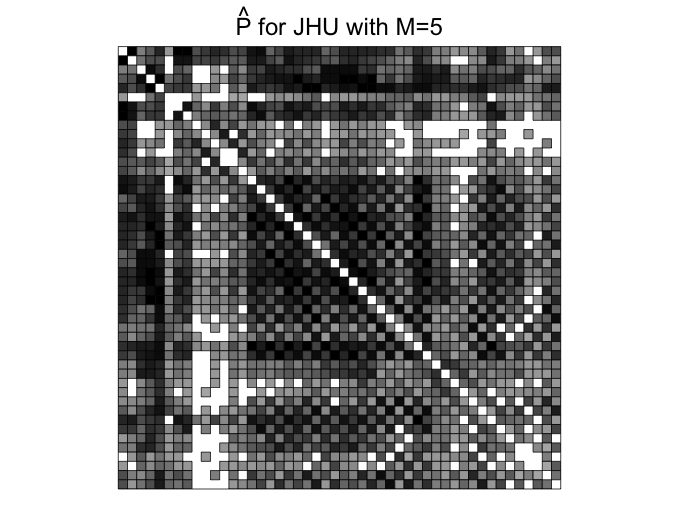
\includegraphics[width=1.2\linewidth]{Phat_JHU_m5.png}
%\end{subfigure}
%\caption{Comparison between the mean of 454 graphs $P$ and two estimates $\bar{A}$ and $\hat{P}$ derived from a sample of size $M=5$ from JHU dataset while embedding the graphs into dimension $d=15$ selected by the 3rd elbow of ZG method.}
%\label{fig:adj_JHU_m5}
%\end{figure}
%
%\begin{figure}[!htbp]
%\centering
%\includegraphics[width=1\textwidth]{Vertex_Diff_Phat_desikan.png}
%\caption{Top 5 regions of the brain (vertices in graphs) with largest absolute difference $|\hat{P} - P|$.}
%\label{fig:Vertex_Diff_Phat_desikan}
%\end{figure}
%
%\begin{figure}[!htbp]
%\centering
%\includegraphics[width=1\textwidth]{Edge_Diff_Phat_desikan.png}
%\caption{Top 1\% (49) connections between regions (edges in graphs) with largest absolute difference $|\hat{P} - P|$.}
%\label{fig:Vertex_Diff_Phat_desikan}
%\end{figure}





\section{Application to a Mouse Connectome}

As a further application of low-rank methods, an MRI-DTI mouse brain connectome \cite{Calabrese2015} with N=1 specimen was evaluated.
The data acquisition protocol is described in the appendix, Section~\ref{section:data_mouse}, and resulted in a $296$ weighted, directed graphs with vertices again corresponding to regions in the brain. 
The  296 regions were organized into a multilevel, hierarchical structure. Analysis of the fine-grained and the first level of the hierarchy partitioned the label set into eight superstructures, with four in each hemisphere: forebrain, midbrain, hindbrain, and white matter. 

The original matrix $W\in (\Re^+)^{296\times 296}$ is a weighed adjacency matrix with $W_{ij}$ denoting the number of tracts passing through ROIs $i$ and $j$.
As the original weights had very heavy tails, these weights were transformed by setting$A_{ij}$ was set to $A_{ij}=\log(W_{ij}+1)$ to transform the original weights, which had very heavy tails. This resulted in the weighted adjacency matrix in Figure~\ref{fig:mouse_adj_lr} (a).


\begin{figure}[tbh!]
	\centering
	\includegraphics[width=\linewidth]{mouse_adj_v_Phat.pdf}
	\caption{The left panel shows the original weighted adjacency with weights transformed by the transformation $w\mapsto \log(w+1)$. 
	The right panel shows the rank-7 approximation of this matrix where the rank was chosen using the \cite{zhu2006automatic} method.
	In both panels, dashed lines show the boundaries between the eight different superstructures. }
	\label{fig:mouse_adj_lr}
\end{figure}

Using the procedure described in Algorithm~\ref{algo:basic}, we found a low-rank approximation to the re-weighted matrix $A$.
In this instance, the \cite{zhu2006automatic} procedure resulted in a rank-7 approximation which is shown in the right panel of Figure~\ref{fig:mouse_adj_lr}.
Since the sample size is only one, cross-validation cannot be employed to analyze the prediction performance of the low-rank methods, but visually it appears that the rank-7 approximation captures many of the features in the original adjacency matrix.

As with the human connectome, we sought to understand the relationship between the structure of the graph, as conveyed through the adjacency spectral embedding, and the eight superstructures which partition the regions of the mouse brain.
Panel (a) of Figure~\ref{fig:mouse_ase} shows entries of the four scaled singular vectors  of the weighted adjacency matrix $A$ corresponding to the largest singular values. 
The points are colored according to the four superstructures and the shapes are determined by the hemisphere. 
The ordering of the points groups together nodes in the same superstructure and hemisphere. The second and fourth vectors have structure which correlates closely with the four superstructures and the two hemispheres, respectively.
Additionally, the first vector appears to separate the midbrain from the other three superstructures.

The right panel of Figure~\ref{fig:mouse_ase} shows a scatter plot of the entries of the fourth and second vectors along with the class boundaries for the eight-class quadratic discriminant analysis classifier, which is based on Gaussian mixture models with no constraints on the covariance structure \cite{Hastie2001-qi}.
This classifier achieves a training error rate of $87/296\approx 0.29$.
The error rate is particularly high for the white matter, with $58/60$ vertices being classified incorrectly, meaning that ignoring the white matter, $29/236 \approx 0.12$ vertices were misclassified. 
Panel (c) shows the normalized confusion matrix for the eight classes, indicating that the forebrain and hindbrain classes are well separated while the white matter and midbrain have more substantial overlap.
This matches with the general structure of the white matter which is not defined at the first hierarchical level of the atlas according to spatial structure, while the fore-, mid-, and hind-brain superstructures are.


Finally, as for the eight human superstructures, the same permutation analysis was also performed for the mouse connectome.
%\todo[inline]{are lobes not the same things as superstructures? would a consistent language help with human to mouse parallelism? it is but a question}
Figure~\ref{fig:mouse_violin} shows the violin plots for the metric defined in Eq.~\eqref{eq:test_stat} permuted in the same way as described in the Appendix.
This test again indicates that the eight superstructures are significant even after accounting for the spatial structure of the regions.







\begin{figure*}[tbh!]
	\centering
	\includegraphics[width=\linewidth]{mouse_connectome_ase_w_error_table.pdf}
	\caption{
	% {\bf Latent positions analysis of the mouse connectome}
	Panel (a) shows the entries of the the four scaled singular vectors  of the weighted adjacency matrix $A$ corresponding to largest singular values.
	The ordering of the entries is the same as the ordering in Figure~\ref{fig:mouse_adj_lr}, where vertices in the same superstructures and hemispheres are grouped together. 
	The colors of points denote the superstructures and the shapes denote the hemispheres.
	Panel (b) shows a scatter plot of the the fourth and second singular vectors. 
	The background coloring corresponds to fitting a classifier, based on a mixture of Gaussians, to classify the eight different superstructures.
	Panel (c) shows the normalized confusion matrix for the mixture of Gaussians learned in panel (b).
    Each entry corresponds to the proportion of nodes with a given label that were predicted to be each other label,
    with the true label given by the row and the predicted label given by the column.}
	\label{fig:mouse_ase}
\end{figure*}

\begin{figure}[tbh!]
	\centering
	\includegraphics[width=\linewidth]{mouse_connectome_violin.pdf}
	\caption{
	% {\bf Violin plot for the mouse connectome permutation test.}
	As in Fig.~\ref{fig:violin_plot}, 1000 simulations for each number of flips show that as the number of flips increases, the distribution under the null moves further from the dashed line. This indicates that the latent positions correlate with the superstructures even after conditioning on the spatial structure. Dashed line represents the situation based on true superstructure assignment.   }
	\label{fig:mouse_violin}
\end{figure}







\section{Discussion}\label{sec:discussion}

% In this paper, we propose using low-rank methods to estimate the mean of a collection of graphs.
Motivated by the RDPG model, our methodology takes advantage of the low-rank structure of graphs by applying a low-rank approximation to the entry-wise MLE.
We give a closed form for the asymptotic relative efficiency between the entry-wise MLE $\bar{A}$ and our estimator $\hat{P}$ in the case of a stochastic blockmodel, demonstrating that when the number of vertices $N$ is sufficiently large, low-rank methods provide a substantial improvement.
In particular, for a stochastic blockmodel with fixed number of blocks $K$, block size proportion $\rho$, and number of graphs $M$, the low-rank estimator $\hat{P}$ has MSE which is on the order of $N$ times lower than the MSE for $\bar{A}$.

Moreover, our estimator outperforms the entry-wise MLE in a cross validation analysis of the SWU4 brain graphs and in low- and full-rank simulation settings when $M$ is small.
% @rt: clarify that this is true when M is small
% @ds: revised
These results illustrate that $\hat{P}$ performs well even when the low-rank assumption is violated and that $\hat{P}$ is robust and can be applied in practice.

One of the key observations from our real data analysis was that the largest improvements using the low-rank method occurred when the number of graphs $M$ was small, and that it provided only minor improvements, or even slightly degraded performance, when $M$ was large.
However, even in large scale studies the low-rank methods will be useful for estimating graph means for subpopulations, e.g.\ the population of females over 60 with some college education.
Using the element-wise sample mean for such small strata, which may have fewer than ten subjects, will frequently result in a degradation of performance.
Similarly, \cite{durante2016nonparametric} proposed a Bayesian nonparametric approach for modeling the population distribution of network-valued data which reduces dimensionality via a mixture model and our methods could be easily adapted to those ideas.


%\begin{figure}[!htbp]
%\centering
%\includegraphics[width=.7\linewidth]{eigenvector.pdf}
%\caption{{\bf Heat map of $\hat{X}$.}
%Heat map of $\hat{X}$ with each row to be the estimated latent position for the corresponding vertex. From the second column, we can see a clear distinction of the left and right hemisphere as conveyed in the second dimension.}
%\label{fig:eigenvector}
%\end{figure}


%\begin{figure}[!htbp]
%\begin{center}
%  \includegraphics[height=.4\linewidth]{desikan2a.png}\hspace{-40pt}
%  \includegraphics[height=.4\linewidth]{desikan2b.png}\hspace{-40pt}
%  \includegraphics[height=.4\linewidth]{desikan2c.png}
%\end{center}
%\caption{{\bf Brain colored by the 2nd dimension of $\hat{X}$.}
%We plot the brain using the 2nd dimension of $\hat{X}$. From the figure, we can see a clear distinction of the left and right hemisphere as conveyed in the second dimension.}
%\label{fig:eigenvector_brain}
%\end{figure}


% \subsection{Future Work}
% In this paper, we assume that the adjacency matrix is observed without contamination.
% However, generally there will be noise in practice and accounting for this noise with other more robust methods . With contaminations, robust estimators like ML$q$E is preferred. If an estimator can not only inherit robustness from the robust estimators but also has small variance by taking advantage of the low rank structure of the graphs, it will be very useful.

% Meanwhile, estimating the rank of the graph structure accurately will certainly help improve the performance of the estimator $\hat{P}$. Now we are using Zhu and Ghodsi's method and USVT, but there is still a lot of space for improvement, especially in this particular case.

While the low-rank methods considered in this paper will often offer substantial improvements, further refinements of these methods which account for the particular traits of connectomics data would be useful to improve estimation further.
For example, we assume that the adjacency matrix is observed without contamination, however in practice there will be noise in the observed graph and one may seek to account for this noise with more robust methods.
This may be especially fruitful when each graph has weighted edges and the weights themselves have noisy or heavy-tailed distributions.
Rank-based methods and robust likelihood methods could be very useful in that case \cite{huber2009robust,qin2013maximum}.

 % With contaminations, robust estimators like ML$q$E is preferred. If an estimator can not only inherit robustness from the robust estimators but also has small variance by taking advantage of the low rank structure of the graphs, it will be very useful.

Another issue that arose in the analysis of the connectome dataset was the presence of structural ones in the mean graph for the population.
These structural ones appear since edges between certain regions of the brain are present in all members of the healthy population.
For these always-present edges, the low-rank methods will have non-zero error while the sample mean will always have zero error.
Detecting and incorporating structural ones and zeros could yield methods that share the best elements of both methods considered here.

For the SWU4 dataset, we performed a cross-validation framework and compared the estimates based on a subsample to the mean for the held-out set.
Another option would be to compare the estimates $\bar{A}$ and $\hat{P}$ to the mean for the entire population including the subsample.
Both of these analyses lead to very similar results in the cases presented above, but for various reasons one may prefer one analysis over another.
The cross-validation method is most reasonable from a prediction perspective where prediction about new samples is of interest.
If instead one is interested in learning directly about the mean of a population, especially a finite population, the sub-sampling approach may be the most logical choice.

While in this paper the focus on the estimation of the probability matrix $P$ based on the low-rank structure, many future directions are quite interesting, such as fitting the SBM or clustering the vertices to detect different brain regions.
For example, \cite{abraham2013extracting} introduced a region-extraction approach based on a sparse penalty with dictionary learning; \cite{calhoun2001method} performed independet component analysis of fMRI data to draw group inferences; \cite{wang2017joint} consider a joint embedding model for feature extractions.
In future work, it would be interesting to explore further statistical inferences based on our method.



\section*{Acknowledgments}

% This work is graciously supported by the XDATA program of the Defense
% Advanced Research Projects Agency (DARPA) administered through Air
% Force Research Laboratory contract FA8750-12-2-0303; the DARPA SIMPLEX
% program through SPAWAR contract N66001-15-C-4041; and DARPA GRAPHS
% contract N66001-14-1-4028. We would also like to acknowledge support from NIH through K01 AG041211, and P41 EB015897.

\nocite{gorgolewski2015high,Garyfallidis2014-wg,Anderson2017-ra,behrens2007manual,brown1977means}

\bibliographystyle{IEEEtran}

\bibliography{Bib.bib}


% \begin{IEEEbiography}[{\includegraphics[width=1in,height=1.25in,clip,keepaspectratio]{Tang.jpg}}]
% {Runze Tang} received the BS degree in mathematics and applied mathematics from the University of Science and Technology of China, in 2012, the MSE degree in computer science from the JHU, in 2015, and the PhD degree in applied mathematics and statistics from the JHU, in 2017. His research interests include robust estimation and statistical inference on graphs.
% \end{IEEEbiography}
% \begin{IEEEbiography}[{\includegraphics[width=1in,height=1.25in,clip,keepaspectratio]{Ketcha.jpg}}]
% {Michael Ketcha} is a PhD Candidate in the Department of Biomedical Engineering at JHU. He received his B.S. in biomedical engineering (2014) from JHU. His research focuses on statistical image analysis with applications in medical imaging, image registration, and image-guided surgery.
% \end{IEEEbiography}
% \begin{IEEEbiography}[{\includegraphics[width=1in,height=1.25in,clip,keepaspectratio]{Badea.jpg}}]
% {Alexandra Badea} is an associate professor in the Radiology Department, with a secondary appointment in the Biomedical Engineering Department, at Duke University. She directs the Visual Informatics Core at the Center for in Vivo Microscopy. 
% % Her research has centered on multivariate image based phenotyping, and atlasing.
% She has focused primarily on magnetic resonance imaging and analysis to provide a comprehensive characterization of the brain morphometry, microstructure, and connectivity.
% % Her interests are uncovering the link between imaging changes, genetic and environmental factors; and between imaging and cognitive/behavioral deficits. She is interested in developing multivariate image analysis and predictive modelling approaches to help better understand human disease indirectly through mouse models, as well as directly in the human brain.
%  \end{IEEEbiography}
%  \vskip 0pt
% \begin{IEEEbiography}[{\includegraphics[width=1in,height=1.25in,clip,keepaspectratio]{Calabrese.jpg}}]
% {Evan D.~Calabrese} is a physician scientist and resident physician in the Department of Radiology and Biomedical Imaging at the University of California San Francisco. His research is focused on developing quantitative imaging biomarkers and automated analysis methods for assessing brain health and disease.
% \end{IEEEbiography}
% \begin{IEEEbiography}[{\includegraphics[width=1in,height=1.25in,clip,keepaspectratio]{Margulies.jpg}}]{Daniel S. Margulies} is a permanent researcher with the Centre national de la recherche scientifique (CNRS) in Paris. He previously led the Neuroanatomy \& Connectivity Research Group at the Max Planck Institute for Human Cognitive and Brain Sciences in Leipzig. His research primarily investigates cortical organization as measured with intrinsic fluctuations in functional MRI data.
% \end{IEEEbiography}
% \begin{IEEEbiography}[{\includegraphics[width=1in,height=1.25in,clip,keepaspectratio]{Vogelstein.png}}]{Joshua T.~Vogelstein} received a B.S degree from the Department of Biomedical Engineering (BME) at Washington University in St. Louis, MO in 2002, a M.S. degree from the Department of Applied Mathematics \& Statistics (AMS) at JHU in 2009, and a Ph.D. degree from the Department of Neuroscience at JHU in 2009. He is currently an Assistant Professor in BME at JHU.
% % and core faculty in the Institute for Computational Medicine and the Center for Imaging Science, and a member of the Kavli Neuroscience Discovery Institute. 
% % He married my kindergarten sweetheart in the summer of 2014. 
% His research interests include computational statistics, focusing on big data, % wide data, and icky data, 
% especially in neuroscience and connectomics.
% \end{IEEEbiography}
% \begin{IEEEbiography}[{\includegraphics[width=1in,height=1.25in,clip,keepaspectratio]{Priebe.jpg}}]
% {Carey E. Priebe} received the BS degree in mathematics from Purdue University, in 1984, the MS degree in computer science from San Diego State University, in 1988, and the PhD degree in information technology from George Mason University, in 1993. % From 1985 to 1994, he worked as a mathematician and scientist in the US Navy research and development laboratory system. 
% He is currently a professor in the Department of Applied Mathematics and Statistics, JHU. %, with joint appointments in Computer Science and Electrical Engineering. 
% His research interests include computational statistics, pattern recognition, and high-dimensional and graph data.
% He is a Senior Member of the IEEE. % a Lifetime Member of the Institute of Mathematical Statistics, an Elected Member of the International Statistical Institute, and a Fellow of the American Statistical Association.
% \end{IEEEbiography}
% \begin{IEEEbiography}[{\includegraphics[width=1in,height=1.25in,clip,keepaspectratio]{DLSussman.jpg}}]{Daniel L. Sussman} received the BA degree in mathematics from Cornell University, in 2008, and the PhD degree in Applied Mathematics and Statistics from JHU, in 2014. From 2014 to 2016 he worked as a postdoctoral fellow at the Harvard University Statistics Department. He is currently an Assistant Professor in the Mathematics and Statistics Department at Boston University. His research interests include spectral methods, multiple graph inference, graph matching, and connectomics.
% \end{IEEEbiography}




\clearpage
\pagenumbering{arabic}
\setcounter{page}{1}
\appendices


\section{Methods}
\label{sec:method}

\subsection{Algorithm for Low-rank Approximation}
Here we provide the algorithm for computing a low-rank positive semidefinite approximation of a matrix.

\begin{algorithm}[H]
\caption{Rank-$d$ approximation of a matrix.}
\label{algo:lowrank}
\begin{algorithmic}[1]
\REQUIRE Symmetric matrix $A\in \Re^{N\times N}$, dimension $d\leq N$.
\ENSURE $\mathrm{lowrank}_d(A)\in \Re^{N\times N}$
\STATE Compute the algebraically largest $d$ eigenvalues of $A$, $s_1\geq s_2\geq \dotsc\geq s_d$ and corresponding orthonormal eigenvectors $u_1,u_2,\dotsc,u_d\in \Re^N$;
\STATE $\hat{S} \leftarrow \mathrm{diag}(s_1,\dotsc,s_d)$ and  $\hat{U} \leftarrow [u_1,\dotsc,u_d]$;
\STATE Return $\hat{U}\hat{S}\hat{U}^{\top}$;
\end{algorithmic}
\end{algorithm}


\subsection{Choosing Dimension}
\label{section:dim_select}
Often in dimensionality reduction techniques, the choice for dimension $d$, relies on analyzing the set of the ordered eigenvalues, looking for a ``gap'' or ``elbow'' in the scree-plot. \citeapp{zhu2006automatic} present an automated method for finding this gap in the scree-plot that takes only the ordered eigenvalues as an input and uses Gaussian mixture modeling to find these gaps.
The mixture modeling results in multiple candidate dimensions or elbows, and our analysis indicated that underestimating the dimension is much more harmful than overestimating the dimension.
For this reason, the 3rd elbow was employed in the experiments performed for this work. While \citeapp{zhu2006automatic} only defines the 1st elbow, we define the $s$-th elbow as in Algorithm~\ref{algo:ZG}.

\begin{algorithm}[H]
\caption{Algorithm to compute the Zhu and Ghodsi's elbow}
\label{algo:ZG}
\begin{algorithmic}[1]
\REQUIRE The number of Zhu and Ghodsi's elbow $s$, with eigenvalues $\lambda_1, \dots, \lambda_N$
\ENSURE The $s$-th Zhu and Ghodsi's elbow
\STATE Calculate the 1st elbow $d_1$ based on $\lambda_1, \dots, \lambda_N$ according to \citeapp{zhu2006automatic}
\FOR{$i$ = 2 to s}
	\STATE {Calculate the $i$-th elbow $d_i$ based on $\lambda_{d_{i - 1} + 1}, \dots, \lambda_N$ according to \citeapp{zhu2006automatic}}
\ENDFOR
\end{algorithmic}
\end{algorithm}


Universal Singular Value Thresholding (USVT) is a simple estimation procedure proposed in \citeapp{chatterjee2015matrix} that can work for any matrix that has ``a little bit of structure''.
In the current setting, it selects the dimension $d$ as the number of singular values that are greater than a constant $c$ times $\sqrt{N/M}$.
The specific constant $c$ must be selected carefully based on the mean and variance of the entries, and since  overestimating the dimension was not overly harmful, we chose a relatively small value of $c=0.7$.

Overall, selecting the appropriate dimension is a challenging task and numerous methods could be applied successfully depending on the setting.
On the other hand, in our setting, many dimensions will yield nearly optimal mean squared errors and the two methods did not pick drastically different dimensions.
Thus efforts to ensure the selected dimension is in the appropriate range are more important than finding the best dimension.



\subsubsection{Exploration of Dimension Selection Procedures}\label{sec:dim}

To further investigate the impact of the dimension selection procedures, we also considered all possible dimensions for $\hat{P}$ by ranging $d$ from 1 to $N$.
$\hat{\mathrm{MSE}}$ of $\bar{A}$ and $\hat{P}$ was plotted in Fig.~\ref{fig:realdata}.
The horizontal axis gives dimension $d$, which only impacts $\hat{P}$, which is why estimated MSE of $\bar{A}$ is shown as flat.
When $d$ is small, $\hat{P}$ underestimates the dimension and throws away important information, which leads to relatively poor performance. When $d=N$, $\hat{P}$ is equal to $\bar{A}$, so that the curve for $\hat{\mathrm{MSE}}$ for $\hat{P}$ ends at $\hat{\mathrm{MSE}}(\bar{A})$.
In the figure, a triangle denotes the 3rd elbow found by the Zhu and Ghodsi method, and a square denotes the dimension selected by USVT with threshold 0.7.
% (with largest 95\% confidence interval length to be $3.5$)
% (with largest 95\% confidence interval length to be $0.7$)
Both dimension selection algorithms tend to select dimensions which nearly minimize the mean squared error.
% The standard error for the Zhu and Ghodsi and the USVT methods are about $0.9$ and $0.17$ respectively.


\begin{figure}[!htbp]
\centering
\includegraphics[width=.99\linewidth]{corr_data_MSE_jhu.pdf}\\
\includegraphics[width=.99\linewidth]{corr_data_MSE_desikan.pdf}\\
\includegraphics[width=.99\linewidth]{corr_data_MSE_CPAC200.pdf}
\caption{
% {\bf Comparison of $\hat{\mathrm{MSE}}$ of $\hat{P}$ and $\bar{A}$ for three atlases at three sample sizes for the CoRR data.}
These plots show the mean squared error for $\bar{A}$ (solid line) and $\hat{P}$ (dashed line) for three datasets (JHU, Desikan, and CPAC200) while embedding the graphs into different dimensions and with different sample sizes $M$. The average dimensions chosen by the 3rd elbow of Zhu and Ghodsi is denoted by a triangle
 % (with largest 95\% confidence interval length to be $3.5$),
 and those chosen by USVT with threshold equaling 0.7 is denoted by a square.
% (with largest 95\% confidence interval length to be $0.7$).
 Vertical intervals, visible mainly in the $N=48,70$ and $M=1$ plots, represent the 95\% confidence interval for the mean squared errors.  When $M$ is small, $\hat{P}$ outperforms $\bar{A}$ with a flexible range of the embedding dimension including the average of the dimensions selected by Zhu and Ghodsi and USVT.}
\label{fig:realdata}
\end{figure}

When $M$ is 1 or 5, $\bar{A}$ has large variance which leads to large $\hat{\mathrm{MSE}}$. Meanwhile, $\hat{P}$ reduces the variance by taking advantages of inherent low-rank structure of the mean graph. Such smoothing effect is especially obvious while there is only 1 observation. When $M = 1$, all weights of the graph are either 0 or 1, leading to a very bumpy estimate $\bar{A}$. In this case, $\hat{P}$ smooths the connectomes estimate and improves the performance.
Additionally, there is a large range of dimensions where the performance for $\hat{P}$ is superior to $\bar{A}$.
With a larger $M$, the performance of $\bar{A}$ improves so that its performance is frequently superior but nearly identical to $\hat{P}$.




\subsection{Graph Diagonal Augmentation}
\label{section:diag_aug}
The graphs examined in this work have no self-loops and thus the diagonal entries of the adjacency matrix and the mean graph are all zero.
However, when computing the low-rank approximation, these structural zeros lead to increased errors in the estimation of the mean graph.
While this problem has been investigated in the single graph setting, with multiple graphs, the problem is exacerbated since the variance of the other entries is lower, so the relative impact of the bias in the diagonal entries is higher.
Moreover, the sum of eigenvalues of the hollow matrix will be zero, leading to an indefinite matrix, which violates the positive semi-definite assumption. So it is important to remedy the situation that we don't observe the diagonal entries.

\citeapp{marchette2011vertex}  proposed the simple method of imputing the diagonals to be equal to the average of the non-diagonal entries for the corresponding row, or in equivalently the degree of the vertex divided by $n-1$.
Earlier, \citeapp{scheinerman2010modeling} proposed using an iterative method to impute the diagonal entries.
In this work, these two ideas are combined by first using the row-average method  (see Step 3 of Algorithm~\ref{algo:basic}) and then using one step of the iterative method (see Step 6 of Algorithm~\ref{algo:basic}).
Note that when computing errors, the diagonal entries are omitted since these are known to be zero.

\subsection{Flipping Procedure for Permutation Test}
\label{section:testing}
%
Here the details of the flipping procedure are described for the permutation test mentioned in Section~\ref{section:lobe_structure}.
As mentioned before, there are 10 lobes and 70 regions based on the Desikan atlas.
We say two regions are adjacent if they share a common boundary. Such spatial adjacency is denoted by an adjacency matrix $S$ for the 70 regions, where $S_{ij} = 1$ means region $i$ and region $j$ contain a pair of voxels, $v_i$ and $v_j$, which are spatially adjacent.
If this is true, then region $j$ is defined as a neighbor of region $i$.
The lobe i.d. for region $i$ is denoted by $l_i$.

Now a uniform $1$-flip can  be defined by:
\begin{enumerate}
\item Selecting a pair of adjacent regions (region $i_1$ and region $j_1$) across the boundary of lobes uniformly, i.e. $S_{i_1 j_1} = 1$ and $l(i_1) \ne l(j_1)$;
\item Uniformly selecting another pair of adjacent regions (region $i_2$ and region $j_2$ where $i_1 \ne i_2$ and $j_1 \ne j_2$) across the same boundary of lobes uniformly, i.e. $S_{i_2 j_2} = 1$ and $l(i_1) = l(i_2)$ and $l(j_1) = l(j_2)$;
\item Reassigning region $j_1$ to lobe $l_{i_1}$ and reassign region $i_2$ to lobe $l_{j_2}$.
\end{enumerate}

By this definition, after a uniform $1$-flip, the number of regions in each lobe stays the same, where only two regions are changed to a different lobe.

Then we can define a uniform $k$-flip naturally as sequentially performing uniform $1$-flip $k$ times.
Note that after a uniform $k$-flip, the number of regions in each lobe still stays the same.

In the permutation test, a uniform $k$-flip was applied and the test statistic $T(X, l)$ was calculated based on the lobe assignment after flipping.
The $p$-value is computed as the proportion of uniform $k$-flips with a $T$ value smaller than the $T$ value for the true lobe assignments.

%\subsection{Mean Squared Error and Relative Efficiency}
%\label{section:rel_eff}
%We evaluate our estimators in terms of mean squared error, either $\mathrm{MSE}(\hat{P}_{ij})=\Ex[\hat{P}_{ij}-P]^2$ or $\mathrm{MSE}(\bar{A})=\Ex[\bar{A}_{ij}-P]^2$.
%While we can directly compare the difference in mean squared errors between the two estimators, it is frequently useful to consider the relative efficiency between two estimators.
%In our case, this is $\mathrm{RE}(\bar{A}_{ij},\hat{P}_{ij}) = \frac{\mathrm{MSE}(\hat{P}_{ij})}{\mathrm{MSE}(\bar{A}_{ij})}$, with values above 1 indicating $\bar{A}$ should be preferred while values below 1 indicate $\hat{P}$ should be preferred.
%We also use asymptotic relative efficiency, which is the limit of the relative efficiency as the number of vertices increase to infinity, and the scaled relative efficiency, $N\cdot \mathrm{RE}(\bar{A}_{ij},\hat{P}_{ij}) $ which in our case normalizes the relative efficiency so that the asymptotic scaled relative efficiency is non-zero and finite.
%Relative efficiency is a useful metric for comparing estimators because it will frequently be invariant to the scale of the noise in the problem and hence is more easily comparable across different settings.

\section{Dataset Description}
\label{section:data}

\subsection{Human Connectomes}
\label{section:data_human}

The original dataset is from the Emotion and Creativity One Year Retest Dataset provided by Qiu, Zhang and Wei from Southwest University available at the Consortium for Reliability and Reproducibility (CoRR) \citeapp{zuo2014open,gorgolewski2015high}. It is composed of 235 subjects, all of whom were college students. Each subject underwent two sessions of anatomical, resting state DTI scans, spaced one year apart. Due to incomplete data, only 454 scans are available.

When deriving MR connectomes, the NeuroData team parcellates the brain into groups of voxels as defined by anatomical atlases \citeapp{kiar2016ndmg}. The atlases are defined either physiologically by neuroanatomists (Desikan and JHU), or are generated using an automated segmentation algorithm (CPAC200).
% The graphs we are using are processed by NeuroData team from DTI data of the original dataset generated with different atlases (Desikan, JHU and CPAC200), each containing different region/node definitions.
Once the voxels in the original image space are grouped into regions, an edge is placed between two regions when there is at least one white-matter tract, derived using a tractography algorithm, connecting the corresponding two parts of the brain \citeapp{Garyfallidis2014-wg}.
The resulting graphs are undirected, unweighted, and have no self-loops.

For the Desikan atlas, there are 70 different regions (35 regions for each hemisphere), with each region belonging to a single lobe. 
Three regions of the Desikan atlas per hemisphere (Banks of Superior Temporal Sulcus, Corpus Callosum, and the ``Unknown'' region) 
do not have obvious lobe assignment and were clustered into a new lobe category named ``other'' to resolve this issue.


\subsection{Mouse Connectome}
\label{section:data_mouse}

Images of the fixed specimen were acquired on a 9.4 T small animal magnet using a 3D diffusion weighted imaging sequence. 
120 unique diffusion directions were acquired using a b value of 4000 s/mm2, interleaved with 11 non-diffusion weighted scans. Images were acquired in 235 hours, and reconstructed at 43 micron resolution. The mouse brain was labeled with 296 regions of interest, 148 per hemisphere \citeapp{Anderson2017-ra}. 

To construct a structural connectome of the mouse brain fiber data was reconstructed (max 4 fiber orientations/voxel), then probabilistic tractography was performed using FSL \citeapp{behrens2007manual},
(5000 samples per voxel, 21 $\mu$m step size, 45 degrees curvature threshold). The 296 seed regions had connectivity estimates produced by counting the number of fibers that originate from one region and fall onto all other regions. This was normalized by the volume of the seed region and resulted in a 296x296 weighted, directed graph.




\section{Proofs for Theory Results}
\subsection{Outline for Main Theorems}
\label{section:outline_proof}
Here the proof of Lemma~\ref{lm:VarPhat} is outlined, which provides the approximate MSE of $\hat{P}$ in the stochastic blockmodel case.
The result depends on using the asymptotic results (see Theorem \ref{thm:clt_ext}) for the distribution of eigenvectors from \citeapp{athreya2016limit} which extend to the multiple graph setting in a straightforward way.

The first key observation is that since $\bar{A}$ is computed from iid observations each with expectation $P$, $\bar{A}$ is unbiased for $P$ and $\mathrm{Var}(A_{ij}) = \frac{1}{M}P_{ij}(1-P_{ij})$.
The results of \citeapp{athreya2016limit} provide a central limit theorem for estimates of the latent position in an RDPG model for a single graph. Theorem~\ref{thm:clt_ext} describes important details.
Since the variance of each entry is scaled by $1/M$ in $\bar{A}$, the analogous result for $\bar{A}$ is that the estimated latent positions will follow an approximately normal distribution with variance scaled by $1/M$ compared to the variance for a single graph.

% When comparing two estimators, the first thing we need to consider is consistency.
% It is easy to see that $\bar{A}$ is unbiased as an estimate of $P$.
% Moreover, since two latent positions are conditionally asymptotically independent by extended version of Theorem 1 in \cite{athreya2013limit}, we know $\hat{P}$ is consistent, as well as $\bar{A}$.


% Thus the relative efficiency between $\hat{P}$ and $\bar{A}$, which is equivalent to the ratio of mean square errors in this case, is a good indicate in comparison.

Since $\hat{P}_{ij} = \hat{X}_i^{\top} \hat{X}_j^{\phantom{\top}}$ is a noisy version of the dot product of $\nu_s^{\top} \nu_t^{\phantom{\top}}$ from Section~\ref{section:sbm_rdpg} and each $\hat{X}_i$ is approximately independent and normal, we can use common results for the variance of the inner product of two independent multivariate normals \citeapp{brown1977means}.
After simplifications that occur in the stochastic blockmodel setting, we can derive that the variance of $\hat{P}_{ij}$ converges to $\left( 1/\rho_{\tau_i} + 1/\rho_{\tau_j} \right) P_{ij} (1-P_{ij})/(N \cdot M)$ as $N \rightarrow \infty$.
Since the variance of $\bar{A}_{ij}$ is $P_{ij} (1-P_{ij})/M$, the relative efficiency between $\hat{P}_{ij}$ and $\bar{A}_{ij}$ is approximately $(\rho_{\tau_i}^{-1} + \rho_{\tau_j}^{-1})/N$ when $N$ is sufficiently large.


\subsection{Proof Details}
Here the proofs are presented of the results in Section~\ref{section:theoretical_result}. To keep the ideas clear and concise, some details are removed, which are only slight changes to previous works.
We assume the block memberships $\tau_i$ are drawn iid from a categorical distribution with block membership probabilities given by $\rho\in[0,1]^K$ where $\sum_i \rho_i =1$.
We will also assume that for a given $N$, the block memberships are fixed for all graphs.

We denote matrix of between-block edge probabilities by $B = \nu \nu^{\top} \in[0,1]^{K\times K}$ which we assume has rank $K$ and is positive definite.
By definition, the mean of the collection of graphs generated from this SBM is $P$, where $P_{ij} = B_{\tau_i, \tau_j}$.

We observe $M$ graphs on $N$ vertices $A^{(1)}, \cdots, A^{(M)}$ sampled independently from the SBM conditioned on $\tau$.
Define $\bar{A} = \frac{1}{M} \sum_{t=1}^M A^{(t)}$. Let $\hat{U} \hat{S} \hat{U}^{\top}$ be the best rank-$d$ positive semidefinite approximation of $\bar{A}$, then we define $\hat{P} = \hat{X} \hat{X}^{\top}$, where $\hat{X} = \hat{U} \hat{S}^{1/2}$.




The proofs presented here will rely on a central limit theorem developed in \citeapp{athreya2016limit}.
The theorem was modified slightly to account for the multiple graph setting and is presented in the special case of the stochastic blockmodel.

\begin{theorem}[Corollary of Theorem 1 in \citeapp{athreya2016limit}]\label{thm:clt_ext}
  In the setting above, let $X=[X_1,\dotsc,X_N]^{\top}\in\Re^{N\times d}$ have row $i$ equal to $X_i=\nu_{\tau_i}$ (recall that $\tau_i$ are drawn from $[K]$ according to the probabilities $\rho$).
	Then there exists an orthogonal matrix $W$ such that for each row $i$ and $j$ and any $z \in \Re^{d}$, conditioned on $\tau_i=s$ and $\tau_j=t$,
  \begin{equation}
    \label{eq:4}
    \begin{split}
    &\Pr\left\{\sqrt{N}( W \hat{X}_i - \nu_s ) \leq z, \sqrt{N}( W \hat{X}_j - \nu_t) \leq z'\right\}\\
    =&  \Phi(z, \Sigma(\nu_s)/M)  \Phi(z', \Sigma(\nu_t)/M) +o(1)\end{split}
  \end{equation}
  where $\Sigma(x) =\Delta^{-1}\Ex[ X_j X_j^\top(x^\top X_j -(x^\top
  X_j)^2)]\Delta^{-1}$ and $\Delta=\Ex[ X_1 X_{1}^{T}]$ is the second
  moment matrix, with all expectations taken unconditionally.
  The function $\Phi$ is the cumulative distribution function for a multivariate normal with mean zero and the specified covariance, and $o(1)$ denotes a function that tends to zero as $N\to \infty$.
\end{theorem}
The proof of this result follows very closely the proof of the result in the original paper with only slight modifications for the multiple graph setting.

We now prove a technical lemma which yields the simplified form for the variance under the stochastic blockmodel.

\begin{lemma}
\label{lm:mseForm}
In the same setting as Theorem~\ref{thm:ARE}, for any $1 \le s, t \le K$:
\[
	\nu_s^{\top} \Sigma(\nu_t) \nu_s^{\phantom{\top}} = \frac{1}{\rho_s} \nu_s^{\top} \nu_t^{\phantom{\top}} (1- \nu_s^{\top} \nu_t).
\]
\end{lemma}
\begin{proof}
Under the stochastic blockmodel with parameters $(B, \rho)$, we have $X_i \stackrel{iid}{\sim} \sum_{k=1}^K \rho_k \delta_{\nu_k}$, where $\nu = [\nu_1, \cdots, \nu_K]^{\top}$ satisfies $B = \nu \nu^{\top}$. Without loss of generality, it can be assumed that $\nu = U S$ where $U = [u_1, \cdots, u_K]^{\top}$ is orthonormal in columns and $S$ is a diagonal matrix. Here it can be concluded that $\nu_s^{\top} = u_s^{\top} S$. Defining $R = \text{diag}(\rho_1, \cdots, \rho_K)$, allows
\[
	\Delta = \Ex[X_1 X_1^{\top}] = \sum_{k=1}^K \rho_k \nu_k \nu_k^{\top} = \nu^{\top} R \nu = S U^{\top} R U S.
\]
Thus
\begin{align*}
	\nu_s^{\top} \Sigma(\nu_t) \nu_s = &
     \sum_{k=1}^K \nu_s^{\top} \Delta^{-1} \rho_k \nu_k \nu_k^{\top} \Delta^{-1} \nu_s (\nu_t^{\top} \nu_k)(1 - \nu_t^{\top} \nu_k) \\
    % = & \sum_{k=1}^K \rho_k (\nu_s^{\top} \Delta^{-1} \nu_k) (\nu_k^{\top} \Delta^{-1} \nu_s) \nu_t^{\top} \nu_k (1 - \nu_t^{\top} \nu_k) \\
    = & \sum_{k=1}^K \rho_k (u_s^{\top} U^{\top} R^{-1} U u_k)^2 (\nu_t^{\top} \nu_k) (1 - \nu_t^{\top} \nu_k) \\
    = & \sum_{k=1}^K \rho_k (e_s^{\top} R^{-1} e_k)^2 (\nu_t^{\top} \nu_k) (1 - \nu_t^{\top} \nu_k) \\
    = & \sum_{k=1}^K \rho_k \delta_{sk} \rho_s^{-2} (\nu_t^{\top} \nu_k) (1 - \nu_t^{\top} \nu_k) \\
    = & \frac{1}{\rho_s} \nu_t^{\top} \nu_s (1 - \nu_t^{\top} \nu_s)
\end{align*}
\end{proof}

% \subsection{Parameter Setting}
% Under SBM($B, \rho$) with $n$ vertices and $K$ blocks, we have the $d$-dimensional latent position $X_i \stackrel{iid}{\sim} \sum_{k=1}^K \rho_k \delta_{\nu_k}$, where $d = \mathrm{rank}(B) \le K$ and $\nu = [\nu_1, \cdots, \nu_K]^T \in \Re^{K \times d}$ satisfying $B = \nu \nu^T$. Define the block assignment $\tau$ such that $\tau_i = k$ if and only if $X_i = \nu_k$. Let $P = X X^T$ where $X = [X_1, \cdots, X_n]^T$.
% Here we assume that the second moment matrix for $X_i$, $\Delta = E[X_i X_i^T]$, is diagonal without loss of generality. Moreover, we assume that the eigenvalues of $\Delta$ are distinct and positive for the remainder of this work.

% First draw $\tau \in [K]^n$ from the multinomial distribution with parameter $\rho$. Then we sample $m$ conditionally i.i.d.~graphs $A^{(1)}, \cdots, A^{(m)}$ such that $A^{(t)}_{ij}|\tau \stackrel{ind}{\sim} Bern(P_{ij})$ for each $1 \le t \le m$, $1 \le i, j \le n$.



% \subsection{Asymptotic Relative Efficiency}

% When two reasonable estimators $S$ and $T$ of the parameter $\theta$ are considered, we always want to know which one is preferred. When both of them are unbiased, the one with a smaller variance would be more efficient. So if $\{S_n\}$ and $\{T_n\}$ are asymptotic unbiased for $\theta$, then define the asymptotic relative efficiency of $\{S_n\}$ with respect to $\{T_n\}$ to be
% \[
% 	\mathrm{ARE}(S_n, T_n) = \lim_{n \rightarrow \infty} \frac{Var(T_n)}{Var(S_n)}.
% \]
% An extended version of ARE is that, when $\{S_n\}$ and $\{T_n\}$ are sequences of estimators for $\theta$ (not necessarily to be asymptotic unbiased), then define the asymptotic relative efficiency of $\{S_n\}$ with respect to $\{T_n\}$ to be
% \[
% 	\mathrm{ARE}(S_n, T_n) = \lim_{n \rightarrow \infty} \frac{Var(T_n)/E[T_n]^2}{Var(S_n)/E[S_n]^2}.
% \]


\begin{lemma}[Lemma~\ref{lm:VarPhat}]
In the same setting as above, for any $i, j$, conditioning on $X_i = \nu_{\tau_i}$ and $X_j = \nu_{\tau_j}$:
\[
	\lim_{N \to \infty} N \cdot \mathrm{Var}(\hat{P}_{ij}) =
    \frac{1/\rho_{\tau_i} + 1/\rho_{\tau_j}}{M} P_{ij} (1 - P_{ij}).
\]
And for $N$ large enough, conditioning on $X_i = \nu_{\tau_i}$ and $X_j = \nu_{\tau_j}$:
\[
	\Ex[(\hat{P}_{ij} - P_{ij})^2] \approx
    \frac{1/\rho_{\tau_i} + 1/\rho_{\tau_j}}{M N} P_{ij}(1-P_{ij}).
\]
\end{lemma}
\begin{proof}
% In Athreya et al. (2013), Theorem 4.8 states that conditioned on $X_i = \nu_k$, there
% exists a sequence of orthogonal matrices $W_n$ converging to the identity almost surely such that
% $P \left( \sqrt{n} (W_n \hat{X}_i - \nu_k) \le z | X_i = \nu_k \right) \rightarrow \Phi(z, \Sigma(x_i))$ as $n \rightarrow \infty$, where $\Sigma(x) = \Delta^{-1} E[X_j X_j^T (x^T X_j)(1 - x^T X_j)] \Delta^{-1}$, $\Delta = E[X_1 X_1^T]$ and $\Phi(z, \Sigma)$ denotes the cumulative distribution function for the multivariate normal, with mean zero and covariance matrix $\Sigma$, evaluated at $z$. Thus the sequence of random variables $\sqrt{n}(W_n \hat{X}_i - \nu_k)$ converges in distribution to a normal distribution.
Conditioned on $X_i = \nu_k$, we have by Theorem~\ref{thm:clt_ext},
\[
	\Ex[W \hat{X}_i] = \nu_k+o(1)
\]
and
\[
	N \cdot \mathrm{Cov}(W \hat{X}_i, W_n \hat{X}_i) = \Sigma(\nu_k)/M.
\]

% The results above are actually based on the \href{https://www.overleaf.com/2962543bbfkxq}{extended version of Avanti's CLT}.

Also, Corollary 3 in \citeapp{athreya2016limit} says $\hat{X}_i$ and $\hat{X}_j$ are asymptotically independent. Thus, conditioning on $X_i = \nu_s$ and $X_j = \nu_t$, we have $\lim_{N\to\infty}\Ex[\hat{X}_i^{\top} \hat{X}_j] = \lim_{N\to\infty}\Ex[(W_N \hat{X}_i)^{\top}] \Ex[W_N \hat{X}_j] = \nu_s^{\top} \nu_t = P_{ij}$.

Since $\hat{P}_{ij} = \hat{X}_i^{\top} \hat{X}_j$ is a noisy version of the dot product of $\nu_s^{\top} \nu_t$, combined with Lemma~\ref{lm:mseForm} and the results above, by Equation 5 in \citeapp{brown1977means}, conditioning on $X_i = \nu_s$ and $X_j = \nu_t$:
\[
	\Ex[\hat{X}_i^{\top} \hat{X}_j] = \Ex[(W_N \hat{X}_i)^{\top}] \Ex[W_N \hat{X}_j] = \nu_s^{\top} \nu_t+o(1) = P_{ij}+o(1)
\]
and
\begin{align*}
	& N \cdot \mathrm{Var} (\hat{P}_{ij}) \\
    = & \frac{1}{M} \left( \nu_s^{\top} \Sigma(\nu_t) \nu_s + \nu_t^{\top} \Sigma(\nu_s) \nu_t^{\top} \right)
    + \frac{1}{M^2 N} \left( tr(\Sigma(\nu_s) \Sigma(\nu_t)) \right) +o(1)\\
    = & \frac{1}{M} \left( \nu_s^{\top} \Sigma(\nu_t) \nu_s + \nu_t^{\top} \Sigma(\nu_s) \nu_t^{\top} \right)+o(1) \\
    = & \frac{1/\rho_s + 1/\rho_t}{M} P_{ij}(1-P_{ij}) + o(1).
\end{align*}
Since $\hat{P}_{ij} = \hat{X}_i^{\top} \hat{X}_j$ is asymptotically unbiased for $P_{ij}$, when $n$ is large enough:
\[
    \Ex[(\hat{P}_{ij} - P_{ij})^2] = \mathrm{Var}(\hat{P}_{ij}) \approx
    \frac{1/\rho_s + 1/\rho_t}{M N} P_{ij}(1-P_{ij})+o(1).
\]
\end{proof}

We now prove Theorem~\ref{thm:ARE}
\begin{proof}[Proof of Theorem~\ref{thm:ARE}]
Combining the MSE result of $\bar{A}_{ij}$
\[
    \Ex[(\bar{A}_{ij} - P_{ij})^2] = \frac{P_{ij}(1-P_{ij})}{M},
\]
and Lemma \ref{lm:VarPhat}, i.e. for large enough $N$,
\[
    \Ex[(\hat{P}_{ij} - P_{ij})^2] \approx
    \frac{1/\rho_{\tau_i} + 1/\rho_{\tau_j}}{M N} P_{ij}(1-P_{ij}),
\]
and therefore there is a large enough $N$,
\[
	    \mathrm{RE}(\bar{A}_{ij}, \hat{P}_{ij}) %= \frac{\mathrm{MSE}(\hat{P}_{ij})}{\mathrm{MSE}(\bar{A}_{ij})}
	    = \frac{\Ex[(\hat{P}_{ij} - P_{ij})^2]}{\Ex[(\bar{A}_{ij} - P_{ij})^2]}
	    \approx \frac{1/\rho_{\tau_i} + 1/\rho_{\tau_j}}{N}.
\]
And the ARE result follows directly by taking the limit of RE as $N\to \infty$.
\end{proof}



% \begin{theorem}
% \label{thm:ARE}
% For any $i$ and $j$, conditioning on $X_i = \nu_{\tau_i}$ and $X_j = \nu_{\tau_j}$, we have
% \[
% 	\mathrm{ARE}(\bar{A}_{ij}, \hat{P}_{ij}) = 0.
% \]
% And for $n$ large enough, conditioning on $X_i = \nu_{\tau_i}$ and $X_j = \nu_{\tau_j}$, we have
% \[
% 	\mathrm{RE}(\bar{A}_{ij}, \hat{P}_{ij}) \approx
%     \frac{1/\rho_{\tau_i} + 1/\rho_{\tau_j}}{n}.
% \]
% \end{theorem}
% \begin{proof}
% Since $A^{(t)}_{ij}$ ($1 \le t \le m$) are i.i.d. Bernoulli random variables with parameter $P_{ij}$, we have
% \[
% 	\mathrm{Var}(\bar{A}_{ij}) = \frac{1}{m} P_{ij} (1 - P_{ij}).
% \]
% Combined with Lemma \ref{lm:VarPhat}, we have
% \[
% 	\mathrm{ARE}(\bar{A}_{ij}, \hat{P}_{ij})
%     = \lim_{n \to \infty} \frac{\mathrm{Var}(\hat{P}_{ij})}{\mathrm{Var}(\bar{A}_{ij})}
%     = 0.
% \]
% For $n$ large enough, conditioning on $X_i = \nu_{\tau_i}$ and $X_j = \nu_{\tau_j}$, we have
% \begin{align*}
% 	\mathrm{RE}(\bar{A}_{ij}, \hat{P}_{ij}) = & \frac{E[(\bar{A}_{ij} - P_{ij})^2]}{E[(\hat{P}_{ij} - P_{ij})^2]} \\
%     \approx & \frac{\mathrm{Var}(\bar{A}_{ij})}{\mathrm{Var}(\hat{P}_{ij})} \\
%     \approx & \frac{1/\rho_{\tau_i} + 1/\rho_{\tau_j}}{n}
% \end{align*}
% \end{proof}

The proof for Theorem~\ref{thm:ARE} is now a simple application of the above lemmas to the ratio of the mean squared errors for $\bar{A}$ and $\hat{P}$.


\section{SBM Simulations} \label{sec:sbm_sim}


\begin{figure}[!htbp]
    \centering
    \includegraphics[width=1\linewidth]{RE.pdf}
    \includegraphics[width=1\linewidth]{scaled_RE.pdf}
    \caption{
    % {\bf Finite sample relative efficiency simulations. }
    The top panel shows the estimated relative efficiency $\hat{\mathrm{RE}}(\bar{A},\hat{P})$ as a function of $N$ for fixed $M=100$ based on simulations of an SBM.
    For each value of $N$, 1000 Monte Carlo replicates of the SBM from Section~\ref{sec:sbm_sim} estimated the RE.
    Each curve corresponds to an average across vertex pairs corresponding to the three distinct block probabilities $B_{11}$, $B_{12}$, and $B_{22}$ in the two-block SBM.
    Recall that values below 1 indicate that $\hat{P}$ is performing better than $\bar{A}$.
    % The relative efficiencies are all very close so the lines are indistinguishable.
    To distinguish the three curves, the bottom panel shows the corresponding scaled relative efficiencies, $N\cdot \hat{\mathrm{RE}}(\bar{A},\hat{P})$.
    The solid horizontal line indicates the theoretical asymptotic scaled relative. }% , which is  $1/\rho_s+1/\rho_t=4$.}
    % All the curves converge quickly to this theoretical limit. 
    % Different types of dashed lines denote the simulated scaled RE associated with different blocks. Solid line represents the theoretical value for scaled RE. Observe that $N \cdot \mathrm{RE}_{st}(\bar{A}, \hat{P})$ converges to $1/\rho_s + 1/\rho_t = 4$ as expected.}
    \label{fig:RE}
\end{figure}

In this section, the theoretical results from Section~\ref{section:theoretical_result} regarding the relative efficiency between $\bar{A}$ and $\hat{P}$ \textit{via} Monte Carlo simulation experiments in an idealized setting will be illustrated.
These numerical simulations will also allow us to investigate the finite sample performance of the two estimators.
% Note that in Section \ref{sec:sim_iem}, the model assumptions will be broken slightly to run experiment in a more realistic setting.

%\subsubsection{Simulation Setting}
Here, we consider the following 2-block SBM with parameters
\begin{equation*}
B = \begin{bmatrix}
0.42 & 0.2 \\
0.2 & 0.7
\end{bmatrix}
,\qquad \rho = \begin{bmatrix}
0.5 & 0.5
\end{bmatrix}.
\end{equation*}
When calculating $\hat{P}$, the dimension selection step from Algorithm~\ref{algo:basic} is omitted and replaced with the true dimension $d = \mathrm{rank}(B) = 2$.
Note that for large $N$, many dimension selection methods will often correctly select the true dimension \cite{chatterjee2015matrix,Fishkind2012}.
1000 Monte Carlo replicates were performed with the above SBM distribution with $N \in \{30, 50, 100, 250, 500, 1000 \}$

%\subsubsection{Simulation Results}
% $M = 100$ graphs from 1000 Monte Carlo replicates using the above SBM distribution with different numbers of vertices $N \in \{30, 50, 100, 250, 500, 1000 \}$ show the relative efficiency $\mathrm{RE}(\bar{A}_{ij}, \hat{P}_{ij})$ can be estimated since $P$ is known for this simulation.
Since the relative efficiency only depends on the block memberships of the pair $i,j$, letting $D_{st} = \{(i, j): \tau_i=s,\tau_j=t,1 \le i < j \le n\}$, the relative efficiency for each block pair can be estimated using
\[
    \hat{\mathrm{RE}}_{st}(\bar{A},\hat{P}) = \frac{\sum_{(i, j) \in D_{st}} \hat{\mathrm{MSE}}(\hat{P}_{ij})}{\sum_{(i, j) \in D_{st}} \hat{\mathrm{MSE}}(\bar{A}_{ij})}
\]
for $s,t\in\{1,2\}$, where $\hat{\mathrm{MSE}}$ denotes the estimated mean squared error based on the Monte Carlo replicates.
For the remaining simulations and real data analysis, we will always be considering estimated relative efficiency and estimated mean squared error rather than analytic results, and hence we will frequently omit that these are estimated values. % when it is clear from context.
% @rt: i don't like saying that things are "clear", for some readers, it won't be clear.
% @ds: revised

In Fig.~\ref{fig:RE}, we plot the (estimated) relative efficiency (top panel) and the scaled (estimated) relative efficiency (bottom panel), $N \cdot \hat{\mathrm{RE}}_{st}(\bar{A},\hat{P})$.
The different dashed lines denote the RE and scaled RE associated with different block pairs, either $B_{11}$, $B_{12}$, or $B_{22}$.
As expected from Theorem~\ref{thm:ARE}, the top panel indicates that the relative efficiencies are all very close together and much less than 1, decreasing at the rate of $1/N$, indicating that $\hat{P}$ is performing better than $\bar{A}$.

Based on Theorem~\ref{thm:ARE}, the scaled RE converges to $1/\rho_{\tau_i}+1/\rho_{\tau_j}=4$ as $N\to\infty$ for all pairs $i,j$.
This is plotted as a solid line in the bottom panel.
The figure shows that $N \cdot \hat{\mathrm{RE}}_{st}(\bar{A}, \hat{P})$ converges to scaled asymptotic RE quite rapidly.
Error bars were omitted, as the standard errors are very small for these estimates.
% {\color{red} Say something about why $B_{11}, B_{22}>4$ and $B_{12}<4$}

\begin{remark}
%  An intriguing aspect of these finite sample results is that the scaled relative efficiencies behave differently for small graphs with fewer vertices.
For small graphs, the estimates of the edge probabilities for pairs of vertices in different blocks are much better than the estimates for edges within each block.
The reason for this is unclear and could be due to the actual values of the true probability, but it may also be due to the fact that there are approximately twice as many pairs of vertices in different blocks, $N^2/4$, than there are in the same block, $N^2/8-N/4$.
This could lead to an increase in effective sample size which may cause the larger differences displayed in the left parts of Fig.~\ref{fig:RE}.
However, these differences are nearly indistinguishable for unscaled relative efficiency overall.
\end{remark}



% \section{Stochastic Blockmodel Parameter Setting}
% \label{section:SBM_parameters}
% Here the parameters in the stochastic blockmodel example depicted in Figure~\ref{fig:SBM_example} are given.
% It is a 5-block SBM with
% \begin{align*}
% B &= \begin{bmatrix}
% 0.90 & 0.27 & 0.05 & 0.10 & 0.30 \\
% 0.27 & 0.67 & 0.02 & 0.26 & 0.14 \\
% 0.05 & 0.02 & 0.44 & 0.25 & 0.33 \\
% 0.10 & 0.26 & 0.25 & 0.70 & 0.18 \\
% 0.30 & 0.14 & 0.33 & 0.18 & 0.58
% \end{bmatrix},\\
% \rho &= \begin{bmatrix}
% 0.22 & 0.39 & 0.05 & 0.16 & 0.18
% \end{bmatrix}.
% \end{align*}


\section{Synthetic Data Analysis for Full Rank IEM}\label{sec:sim_iem}

While the theory we have developed is based on the assumption that the mean graph is low rank, as we have seen in Section~\ref{sec:corr_data}, $\hat{P}$ can perform well even when this assumption is false.
To further illuminate this point, a synthetic data analysis under a more realistic full-rank independent edge model was performed.
As discussed in Section~\ref{sec:challenge}, the sample mean of the 454 graphs in the Desikan dataset is actually of full rank.
For this simulation, we will use the sample mean as the probability matrix $P$.
A sampling of independent graphs from the full rank IEM with the probability matrix $P$ show that for the synthetic data sets of size $M = 1, 5$, and $10$, $\hat{P}$ performs even better than $\bar{A}$ in the real data experiments. 
Fig.~\ref{fig:sim_desikan} shows the resulting estimated MSE for $\bar{A}$ (solid line) and $\hat{P}$ (dashed line), as a function of the embedding dimension for simulated data based on the full rank probability matrix $P$ shown in the left panel of Fig.~\ref{fig:Matrix_desikan_m5}.
% Vertical lines at each dimension indicate the 95\% confidence intervals for the MSE.
These results are similar to those presented in Section~\ref{sec:corr_data}, though overall $\hat{P}$ performs even better than in the real data experiments.
When $M$ is small, $\hat{P}$ outperforms $\bar{A}$ with a flexible range of embedding dimensions including those selected by the Zhu and Ghodsi method.
On the other hand, when $M$ is large enough, both estimators perform well with the decision between the two being less conclusive.
This simulation again shows the robustness of $\hat{P}$ to deviations from the RDPG model, specifically if the probability matrix is full-rank.

We also note that the finite-sample relative efficiency for this synthetic data is even more favorable to $\hat{P}$ than for the real data, with relative efficiency lower than $1/3$ for $M=1$ in the synthetic data analysis as compared to relative efficiency which were at best around $1/2$ for $M=1$ in the original data.
From this observation, we can postulate that the degradation in the performance of $\hat{P}$ in real data can at least partially be attributed to the fact that the independent edge assumption does not hold for real data.
It also suggests that more elaborate models of connectomes will be valuable for various inferential tasks.


\begin{figure}[!htbp]
\centering
\includegraphics[width=1\linewidth]{sim_desikan.pdf}
\caption{
{\bf Comparison of $\hat{P}$ and $\bar{A}$ for synthetic data analysis.}
As in Fig.~\ref{fig:RE}, this figure shows $\hat{\mathrm{MSE}}$ for $\bar{A}$ (solid line) and $\hat{P}$ (dashed line) for simulated data with different sample sizes $M$ based on the sample mean for the Desikan dataset. Again, the average of dimensions selected by the USVT method (square) and the ZG method (triangle) tend to nearly approximate the optimal dimension.
Overall, the structure of these plots well approximates the structure for the real data indicating that performance for the independent edge model will tend to translate in structure to non-independent edge scenarios.
On the other hand, the relative efficiency $\hat{\mathrm{RE}}(\bar{A},\hat{P})$ is lower for this synthetic data analysis than for the CoRR data.}
\label{fig:sim_desikan}
\end{figure}




\bibliographystyleapp{IEEEtran}

\bibliographyapp{Bib}


\end{document}
